\chapter{Desarrollo}
\label{cap:Desarrollo}

\setlength{\parindent}{0pt}

En este capítulo se hablará del desarrollo de la aplicación (diseño, funcionalidades, librerías, gestión del wallet, documentación\dots) que se ha estado realizando a lo largo del TFG, así como el registro de claves para poder interactuar con la red blockchain que se ha levantado. También, se explicará en que consiste el SDK desarrollado, cuales son sus funcionalidades y como poder utilizarlo en otras aplicaciones Android. \\

El desarrollo de la aplicación móvil, se ha enfocado únicamente a dispositivos Android. Lógicamente, en un futuro, se tendrá que adaptar una aplicación para otros sistemas operativos como iOS. O por el contrario reescribir él código con lenguajes ``cross platform'' para permitir el correcto funcionamiento nativo tanto en Android como en iOS, una buena opción es utilizar \textbf{flutter}\cite{flutter}.






% ##################################################
% ##################################################
\section{Arquitectura de la Aplicación}

Recordemos un poco el esqueleto del proyecto ``Estublock''. Se ha decidido crear varios componentes modulares soportados por APIs, así cambios en el código de un componente no afectan al resto. El proyecto dispone de tres APIs diferentes. Tenemos primero la API que comunica con el servidor que tiene ejecutando la base de datos, luego la API que trata algunos datos con la red blockchain que se ha levantado. Y por último, una API intermedia que es con la que se comunica el dispositivo móvil para centralizar las llamadas, quitarle trabajo de computo al móvil y a la aplicación. Sin embargo, recordemos que el dispositivo móvil también hará llamadas directamente a la red blockchain a través del \hyperref[sec:SDK]{SDK}. La arquitectura queda como se muestra en la figura \ref{fig:estublockArch}. \\

El dispositivo móvil se comunica entonces con la api de microservicios con la ayuda de dos librerías que veremos más en profundidad en el apartado de \hyperref[sec:Codigo]{Codigo}, esta API a su vez se comunica con la API de la base de datos o de la red blockchain según la operación que se haya especificado y estas se comunican con el servidor postgresql para la base de datos y la red de quorum para la blockchain. \\

\begin{figure}[h!]
  \centering
  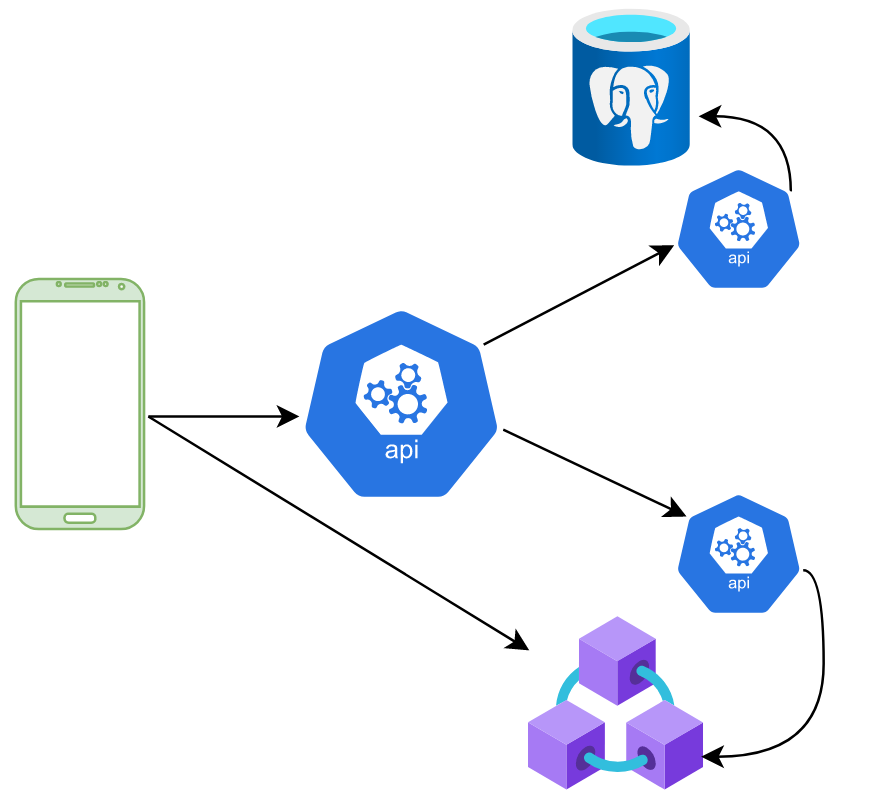
\includegraphics[width=0.35\linewidth]{figs/Desarrollo/Arquitectura}
  \caption[Arquitectura]{Arquitectura Completa del proyecto}
  \label{fig:estublockArch}
\end{figure}







% --------------------------------------------------
\clearpage
\section{Interaz de Usuario}

La interfaz de usuario es donde los usuarios interaccionan con la aplicación. Son las ventanas, botones, pantallas con las que el usuario interacciona. Deben tener un diseño intuitivo, fácil, que brinde una experiencia positiva. A más fácil de entender, mejor. Existen tres grandes tipos de interfaces de usuario, la interfaz de lenguaje natural, es la ideal y el sueño de todo usuario, pues permite comunicar humano y máquina con lenguaje natural. Un ejemplo de dispositivo que utiliza esta interfaz es \emph{Alexa}, que cuenta con un software basado en modelos acústicos y del lenguaje. El segundo tipo de interfaz es la interfaz de preguntas y respuestas. En esta interfaz se muestra una pregunta al usuario y según su respuesta se actúa de una u otra manera. Un ejemplo de estas interfaces son los software de instalación, como puede ser el instalador de un sistema operativo. Y por último, la interfaz que más nos interesa para este proyecto, la \textbf{interfaz gráfica de usuario}, en inglés ``Graphical User Interface'' o \textbf{GUI}. Esta utiliza gráficos, imágenes, videos, iconos, menús\dots para permitir al usuario interaccionar con la aplicación. 

\subsection{Interfaces Gráficas en Android} \label{sec:GUI}

En Android la interfaz de usuario se construye mediante una jerarquía de objetos, generalmente de tipo \textbf{View y ViewGroup}. Los \emph{View} son componentes con los que el usuario puede interactuar, el usuario puede ver el componente en la pantalla. Sin embargo los \emph{ViewGroup} son un contenedor invisible que define la estructura de objetos \emph{View} y otros \emph{ViewGroup}, un árbol jerárquico puede verse en la figura \ref{fig:interfaz_android}.

\begin{figure}[h!]
  \centering
  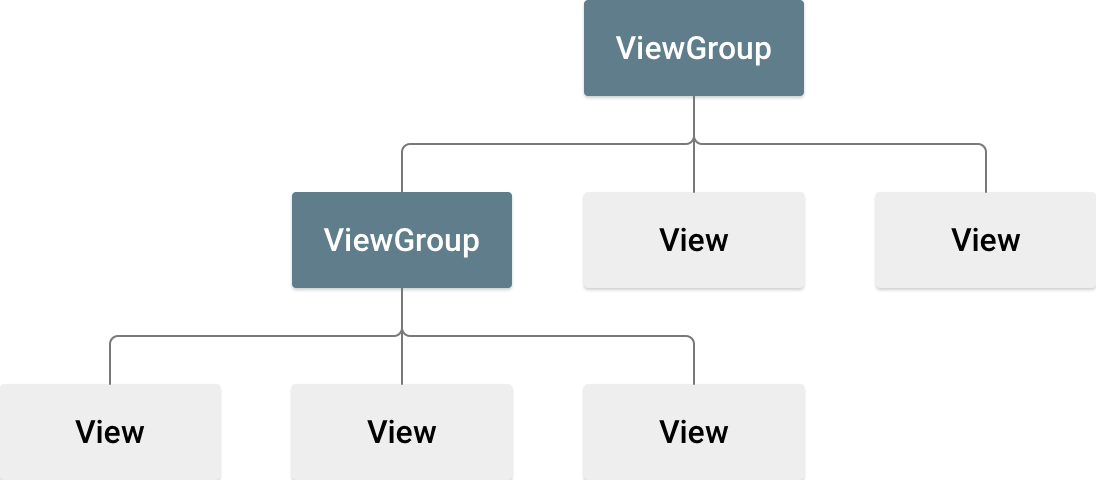
\includegraphics[width=0.6\linewidth]{figs/Desarrollo/Jerarquia}
  \caption[Android Layout]{Jerarquia de una interfaz de Android}
  \label{fig:interfaz_android}
\end{figure}

Los objetos \emph{View} se denominan ``widgets'' y pueden ser Botones, Textos, ``Switch'', ``ScrollView''\dots Los objetos \emph{ViewGroup} se denominan ``diseño'' y pueden ser ``LinearLayout'', ``ConstraintLayout''\dots Los diseños se pueden declarar de dos maneras, podemos declararlos con antelación, esto es programar en código XML como queremos que se vea una pantalla. Y también se pueden instanciar desde el código en tiempo de ejecución y modificar datos de la pantalla, o crear nuevos datos que no hay, (los datos pueden ser botones, cajas, menus, desplegables\dots). \\

Para la aplicación, se han usado ambas formas, pues por un lado hay pantallas estáticas, como pueden ser la pantalla de login o registro. En las que se sabe que botones tiene que haber, que textos tiene que mostrar y que diseño tiene con antelación. Pero también hay pantallas en las que se crean botones o texto de forma dinámica, por ejemplo, en pantallas que muestran próximos eventos, se muestra de forma dinámica (según el número de eventos que devuelva la API) más o menos botones. \\

Uno de los puntos fuertes de programar con antelación la interfaz con XML, es que se puede separar la presentación de la app del código que controla los componentes, además, facilita la creación de distintos diseños para diferentes tamaños de pantalla, orientación, colores\dots Es la mejor opción a la hora de crear una interfaz de usuario aunque en ocasiones se requiera de crear o modificar de forma dinámica en tiempo de ejecución algunos elementos. También es habitual crear con XML un diseño estático, y luego modificarlo en tiempo de ejecución según sea necesario accediendo a sus componentes.  

% --------------------------------------------------
\subsection{Diseño de la Interfaz de Estublock}

A la hora de diseñar la aplicación Estublock, se ha buscado un diseño ligero, intuitivo y rápido. Como que tener en cuenta a muchos usuarios, hay que pensar en los posibles problemas de visión, daltonismo, dislexia, evitar que se pueda mal interpretar un botón\dots todo esto para evitar en la medida de lo posible que el usuario se lleve una mala experiencia con la aplicación. Para todo ello, se ha utilizado una herramienta de diseño para prototipos de pantallas y testeo de pantallas llamada \emph{Marvelapp}\cite{marvelapp}. Marvelapp permite diseñar con bastante detalle aplicaciones móvil y web, y además permite enlazar pantallas para probar la efectividad de las pantallas y el entendimiento de las mismas. Marvelapp tiene un gran potencial al permitir diseñar rápidamente pantallas y poder probar su efectividad rápidamente. \\

\subsubsection{Pantalla de Registro}

En la pantalla de registro, se pide al usuario que introduzca sus datos personales. Se comprueba que los datos sean correctos, por ejemplo, al introducir el correo electrónico, un \verb|regex| se encarga de verificar que el correo sea universitario. Los regex evalúan expresiones regulares y se puede buscar con él un patrón como puede ser \verb|@alumnos.upm.es| para verificar que el usuario es por ejemplo un alumno. El regex que se ha utilizado para comprobar el correo se muestra en la figura \ref{fig:regex}. \\

\begin{figure}[h!]
  \centering
  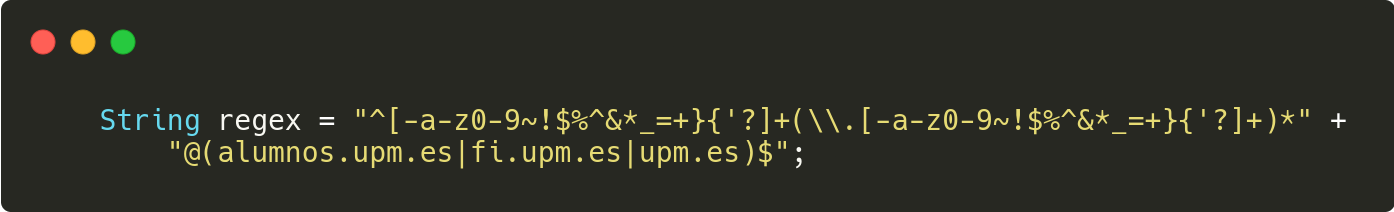
\includegraphics[width=0.9\linewidth]{figs/Desarrollo/Codigo/regex}
  \caption[Android Layout]{Jerarquia de una interfaz de Android}
  \label{fig:regex}
\end{figure}

También, se hace verificación de que la contraseña ha sido escrita correctamente dos veces. Esta es una \textbf{nueva} decisión de diseño, puesto que en un inicio como veremos mas adelante, no se contemplaba en la pantalla de registro pedir la contraseña dos veces. Además, otros cambios que ha sufrido la pantalla de registro es en el número de datos que se le piden al usuario. Se ha eliminado la matrícula, esto es temporal, pues es probable que se añada en el futuro. La principal razón que nos llevó a tomar esta decisión, es que los profesores o ponentes de charlas que fuesen a utilizar esta aplicación, no disponen de matrícula. Solo los estudiantes tienen matrícula. Por otro lado, el nombre y apellidos se piden de forma conjunta, esto también es temporal pues hay que estudiar si van a ser o no datos fundamentales para poder acreditar al alumno la asistencia a un evento, o no es tan importante conocer el primer y segundo apellido del usuario, pues al final lo más importante es el correo electrónico. El diseño con \emph{marvelapp} y el resultado final, pueden encontrarse en la figura \ref{fig:pantalla_registro}

\begin{figure}[hbt]
	\centering
	\begin{subfigure}[b]{0.4\linewidth}
		\centering
        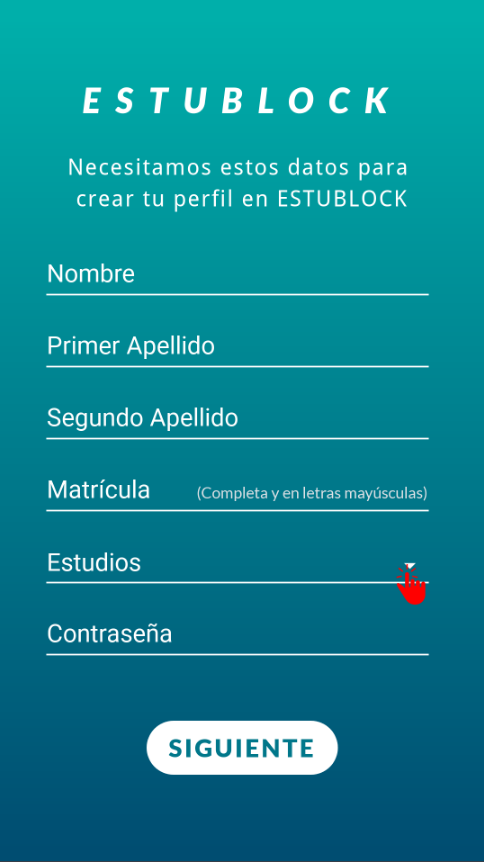
\includegraphics[width=0.5\linewidth]{figs/Desarrollo/Interfaz/marvel_registro}
        \caption[Marvel Registro]{Pantalla de registro de marvelapp}
	\end{subfigure} 
	\begin{subfigure}[b]{0.4\linewidth}
		\centering
        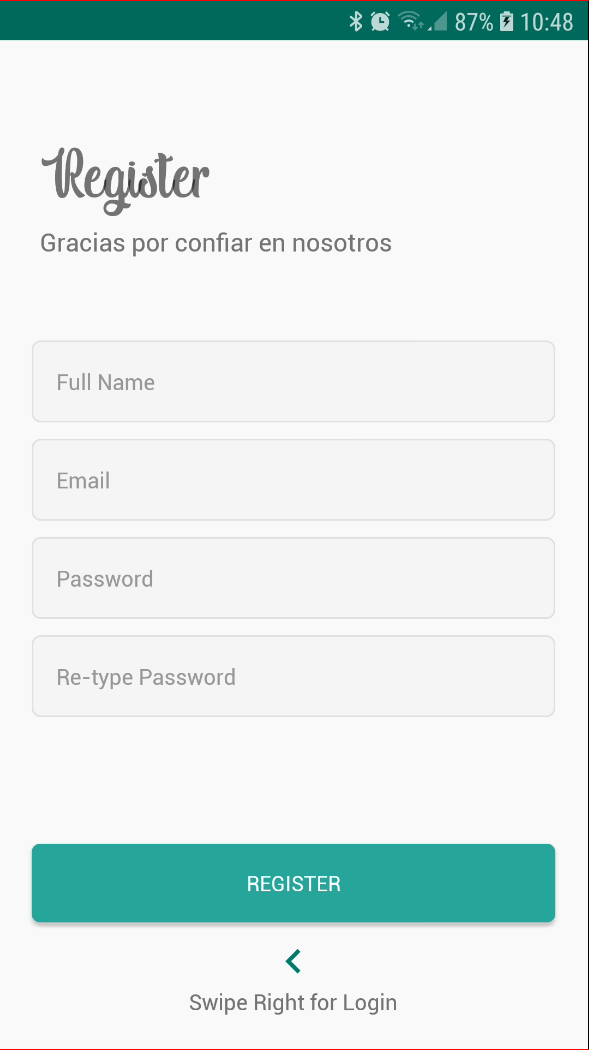
\includegraphics[width=0.5\linewidth]{figs/Desarrollo/Interfaz/estublock_registro}
        \caption[Estublock Registro]{Pantalla de registro de Estublock}
	\end{subfigure} 
	\caption[Pantalla de Registro]{Pantalla de Registro}
	\label{fig:pantalla_registro}
\end{figure}

\subsubsection{Pantalla de Login}

En la pantalla de login, los usuarios pueden iniciar sesión, desbloqueando además su wallet. Este término y sus detalles se verán en el apartado \hyperref[sec:wallet]{Wallet}. Al hacer login, los usuarios solo necesitan introducir el correo electrónico con el que se dieron de alta y la contraseña. Como se puede observar en la figura\ref{fig:login} en \emph{Marvelapp} se añadió la opción de recuperar la contraseña del usuario. Sin embargo, no existe en la versión final. \\

Para poder recuperar la contraseña de un usuario, lo normal en un servicio es enviarle un correo electrónico al usuario (al correo que el usuario utilizaó para darse de alta) y desde ese correo el usuario accede a un portal en el que puede modificar su contraseña. Y la contraseña modificada se pasa por una función \verb|hash|\cite{whatIsHash} y se almacena en una base de datos. En el caso de Estublock, a pesar de poder implementar dicho servicio sin problema, y modificar en la base de datos el hash de la contraseña. No serviría de nada, pues la contraseña que se utiliza para desbloquear y utilizar el wallet no puede ser modificada, si el usuario pierde o se le olvida la contraseña, el wallet queda invalidado. Existen dos principales métodos para recuperar el acceso al wallet, estos se verán en el apartado \hyperref[sec:wallet]{Wallet}. Por lo tanto, ante este problema, la pantalla de login final no tiene opción de recuperar las credenciales por ahora. Pues se puede implementar uno de los métodos de recuperación de wallets disponibles. Tanto la pantalla original como la final se pueden ver en la figura \ref{fig:pantalla_login}. \\

\begin{figure}[hbt]
	\centering
	\begin{subfigure}[b]{0.4\linewidth}
		\centering
        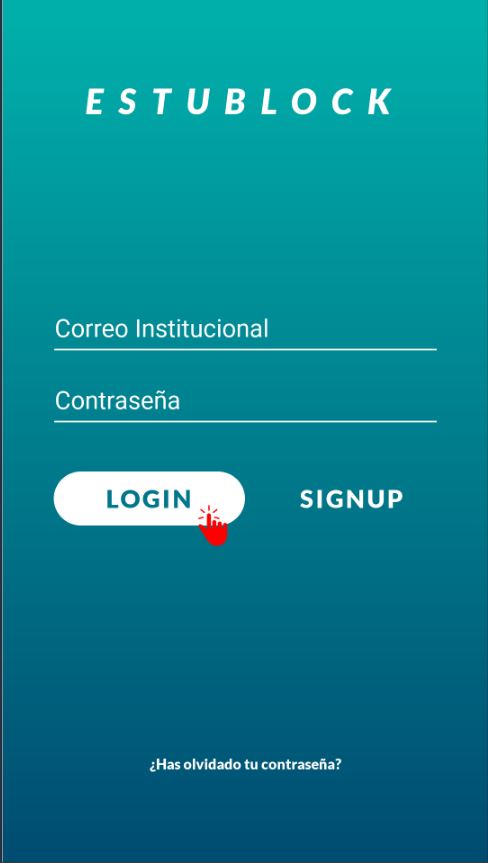
\includegraphics[width=0.5\linewidth]{figs/Desarrollo/Interfaz/marvel_login}
        \caption[Marvel Login]{Pantalla de login de marvelapp}
	\end{subfigure} 
	\begin{subfigure}[b]{0.4\linewidth}
		\centering
        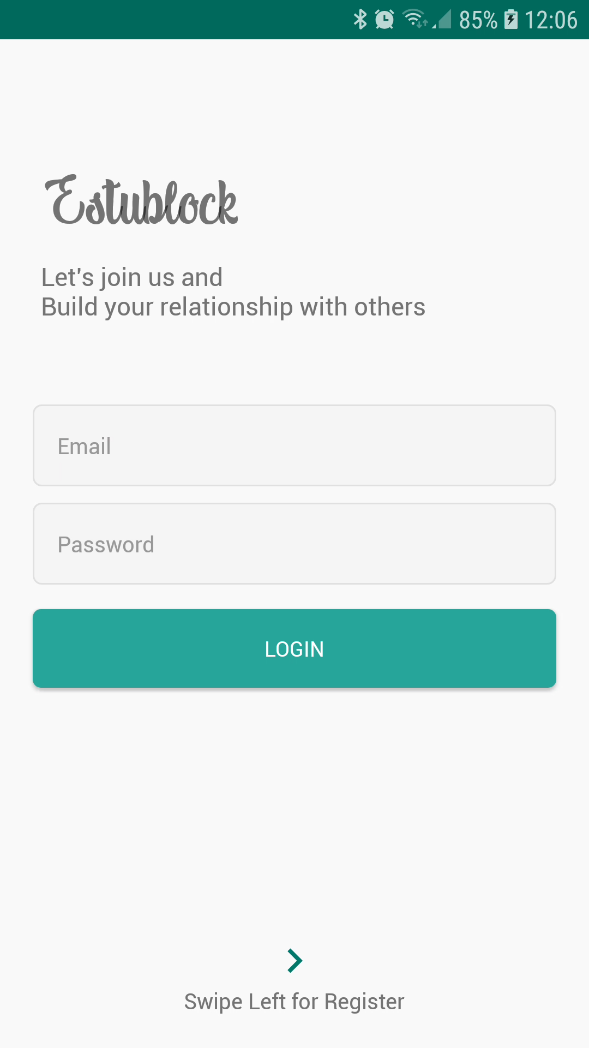
\includegraphics[width=0.5\linewidth]{figs/Desarrollo/Interfaz/estublock_login}
        \caption[Estublock Login]{Pantalla de login de Estublock}
	\end{subfigure} 
	\caption[Pantalla de Login]{Pantalla de Login}
	\label{fig:pantalla_login}
\end{figure}

\subsubsection{Menú Principal}

El menú principal es el corazón de la aplicación. Pues desde ahí se abre camino al resto de funcionalidades de la aplicación. Por un lado es una pantalla importante, pues recoge gran parte de los componentes de la aplicación, pero a su vez, es muy básica y no tiene nada interesante, pues lo único que hace es redirigir al usuario a las funcionalidades disponibles. Estéticamente hablando, la pantalla que se diseño en Marvelapp ha perdido mucho valor visual, pues la pantalla resultante es más básica y menos colorida. Sin embargo, aunque la estética es importante, la funcionalidad principal del menú es redirigir al usuario y esto sí lo hace perfectamente bien. El diseño final así como los botones han sufrido muchos cambios. De hecho, excepto el botón de \emph{asignaturas} el resto de botones es diferente. Esta decisión se ha tomado para agilizar el objetivo principal de la aplicación, es decir, queremos escanear QRs para validar la asistencia de usuarios a eventos. Por tanto, tenemos un botón \emph{crear eventos}, un botón \emph{asistencia} que genera el QR y un botón \emph{Escanear QR} que permite escanear los QR. Desde el menú se puede hacer todo, los cambios se pueden ver en la figura\ref{fig:pantalla_menu}. \\

\begin{figure}[hbt]
	\centering
	\begin{subfigure}[b]{0.4\linewidth}
		\centering
        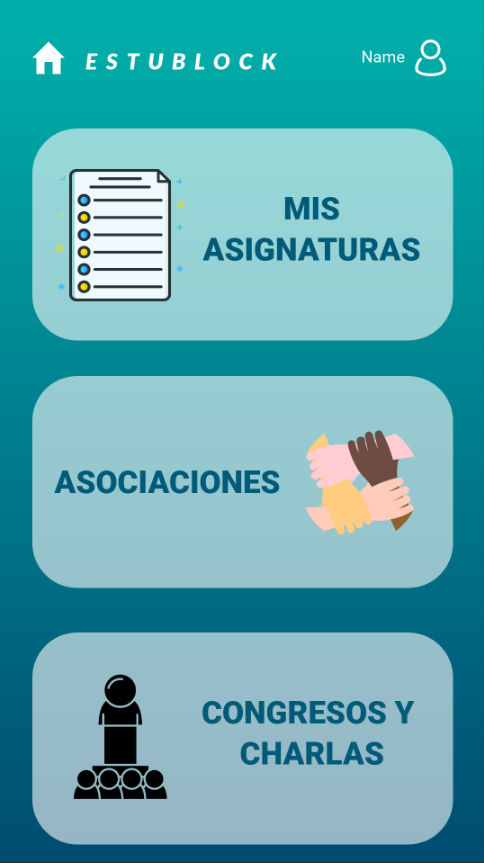
\includegraphics[width=0.5\linewidth]{figs/Desarrollo/Interfaz/marvel_menu}
        \caption[Marvel Menú]{Pantalla de menú de marvelapp}
	\end{subfigure} 
	\begin{subfigure}[b]{0.4\linewidth}
		\centering
        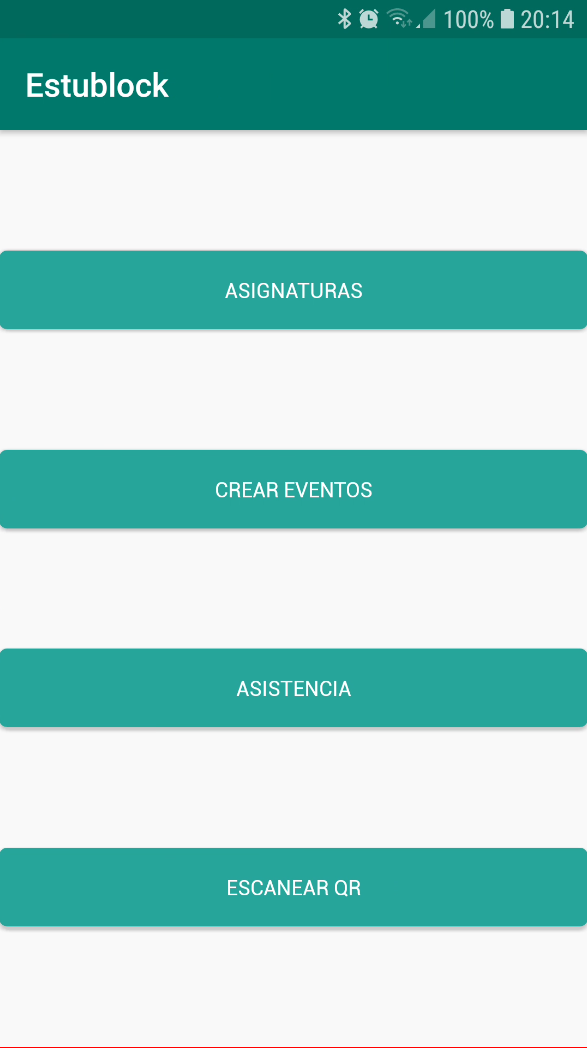
\includegraphics[width=0.5\linewidth]{figs/Desarrollo/Interfaz/estublock_menu}
        \caption[Estublock Menú]{Pantalla de menú de Estublock}
	\end{subfigure} 
	\caption[Pantalla de Menú]{Pantalla de Menú}
	\label{fig:pantalla_menu}
\end{figure}

\subsubsection{Pantalla de Suscripciones}

En la pantalla de suscripciones el usuario puede ver la lista de asignaturas a las que esta suscrito. También se le permite añadir y eliminar asignaturas, para que según avance el curso y vaya aprobando asignaturas pueda no verlas en la lista. Visualmente la pantalla de Marvelapp y la de Estublock han cambiado, pero las funcionalidades. Los que sí se puede destacar, es que se ha puesto en la pantalla de Estublock un botón grande que pone \verb|Añadir| y otro \verb|Eliminar| con esto lo que conseguimos es que el usuario tenga claro donde puede ir a añadir asignaturas o eliminarlas. En la pantalla que se hizo con Marvelapp, el botón de añadir es pequeño y se encuentra en una esquina, y puede no verse con claridad. El diseño de la pantalla queda mostrado en la siguiente figura\ref{fig:pantalla_asignaturas}

\begin{figure}[hbt]
	\centering
	\begin{subfigure}[b]{0.4\linewidth}
		\centering
        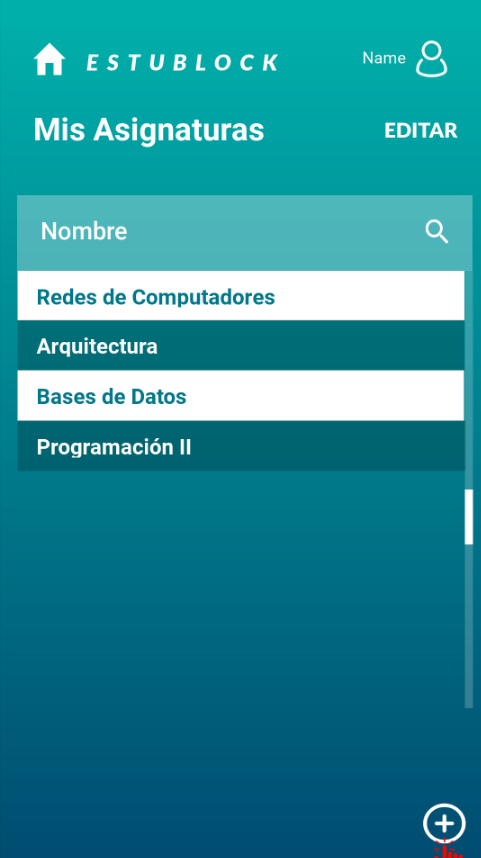
\includegraphics[width=0.5\linewidth]{figs/Desarrollo/Interfaz/marvel_lista_asignaturas}
        \caption[Marvel Asignaturas]{Pantalla de asignaturas de marvelapp}
	\end{subfigure} 
	\begin{subfigure}[b]{0.4\linewidth}
		\centering
        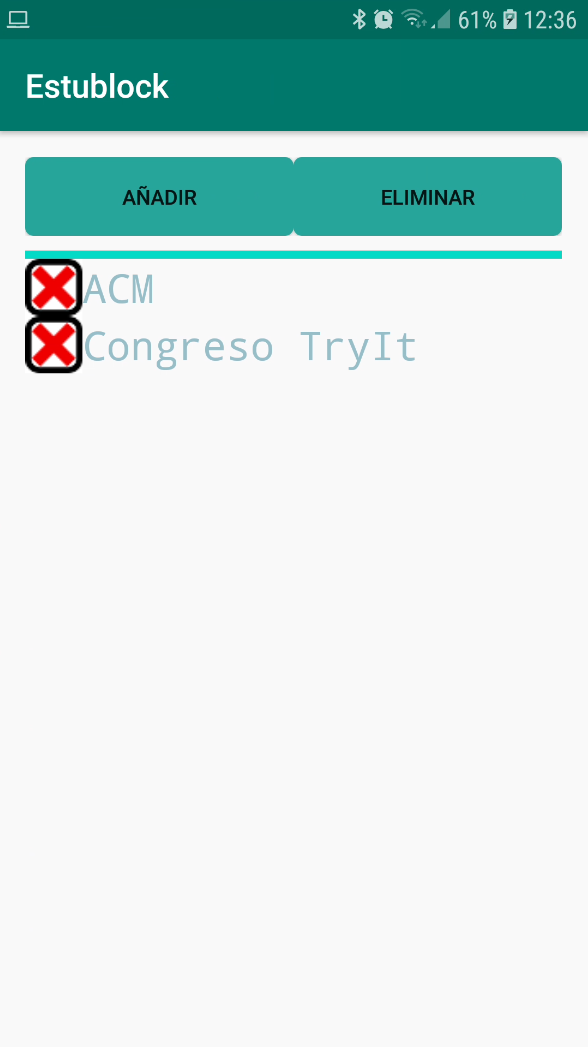
\includegraphics[width=0.5\linewidth]{figs/Desarrollo/Interfaz/estublock_asignaturas_suscritas}
        \caption[Estublock Asignaturas]{Pantalla de asignaturas de Estublock}
	\end{subfigure} 
	\caption[Pantalla de Asignaturas]{Pantalla de Asignaturas}
	\label{fig:pantalla_asignaturas}
\end{figure}

Si el usuario decide añadir nuevas asignaturas a su lista, tendrá que darle al botón de \verb|Añadir|. Esto le lleva a una nueva pantalla en la que se listan todas las asignaturas que hay disponibles para suscribirse. Una vez el usuario selecciona las asignaturas puede proceder a guardarlas. Con respecto al diseño original y al resultado final, caben destacar dos aspectos. El primero es que el botón \verb|Guardar| se ha movido de sitio, no hay ninguna razón especial para esta decisión. Por otro lado, lo que falta es un buscador de asignaturas, este no se ha añadido por ahora, pues no era de crucial importancia al no tener una lista grande de asignaturas disponibles. Sin embrago, es importante que esto se añada en el futuro, pues son muchas las asignaturas que pueden acumularse. El resultado puede verse en \ref{fig:pantalla_añadir_sus}

\begin{figure}[hbt]
	\centering
	\begin{subfigure}[b]{0.4\linewidth}
		\centering
        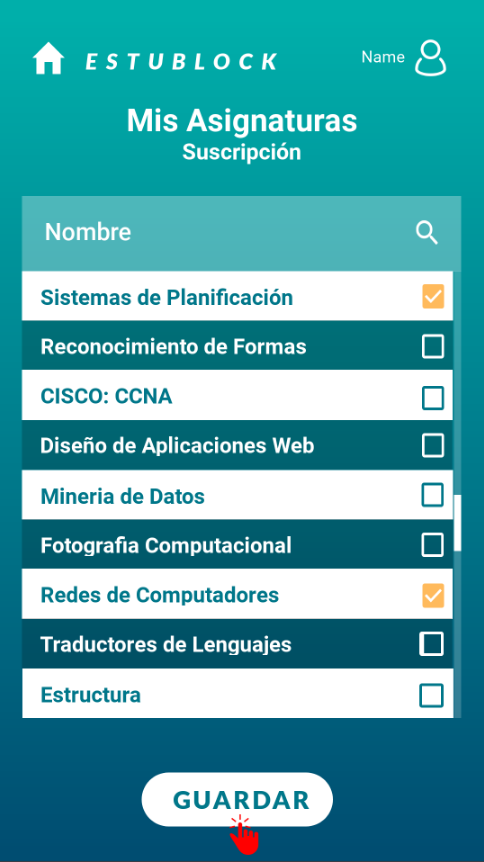
\includegraphics[width=0.5\linewidth]{figs/Desarrollo/Interfaz/marvel_asignaturas}
        \caption[Marvel Suscribirse]{Pantalla de suscripción de marvelapp}
	\end{subfigure} 
	\begin{subfigure}[b]{0.4\linewidth}
		\centering
        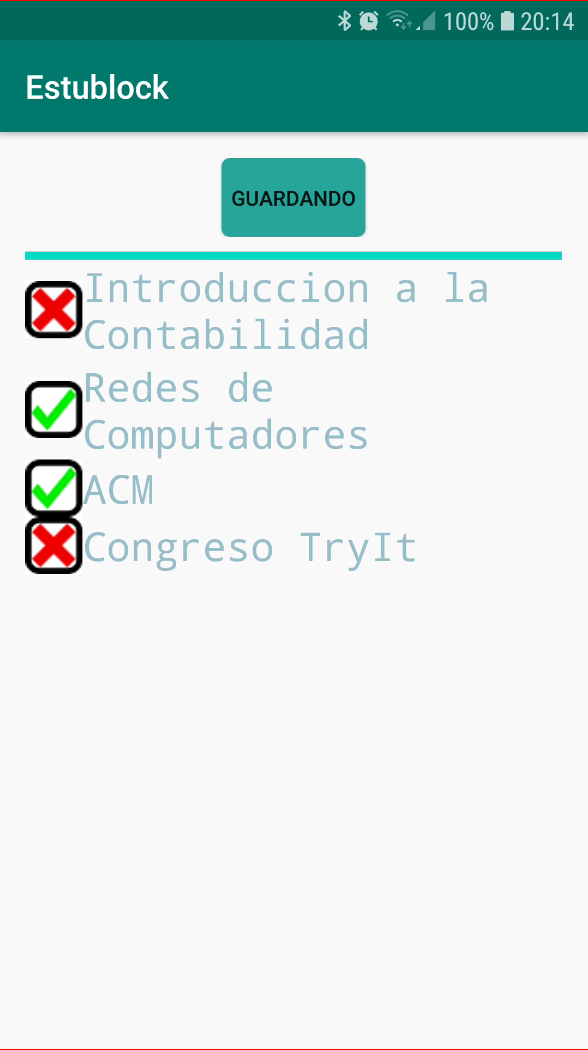
\includegraphics[width=0.5\linewidth]{figs/Desarrollo/Interfaz/estublock_asignaturas}
        \caption[Estublock Suscribirse]{Pantalla de suscripción de Estublock}
	\end{subfigure} 
	\caption[Pantalla de Suscribirse]{Pantalla de Suscribirse}
	\label{fig:pantalla_añadir_sus}
\end{figure}

\subsubsection{Pantalla de Creación de Eventos}

Para llegar a esta pantalla, el usuario tiene que ir desde el menú, a \verb|Crear Evento|, luego se le muestra una pantalla con la lista de asignaturas a las que esta suscrito, y una vez seleccionada la asignatura de la que se quiere crear un evento, se le muestra la pantalla de creación de eventos. En esta pantalla el usuario debe introducir datos sobre el evento como el nombre, fecha, hora, descripción\dots Esta pantalla se ha mantenido muy parecida al diseño realizado con Marvelapp. La única diferencia es que en Marvellapp, el usuario pulsaba \verb|Siguiente| y podía ver un resumen de los datos antes de guardarlos. Se ha decidido eliminar este paso extra, por no aportar nada, pues el usuario puede ver los datos que ha introducido de todos modos en la propia creación del evento, guardando una vez este seguro de los datos elegidos. A continuación se pueden ver unas capturas del resultado \ref{fig:pantalla_crear_evento}, \ref{fig:pantalla_hora}

\begin{figure}[hbt]
	\centering
	\begin{subfigure}[b]{0.4\linewidth}
		\centering
        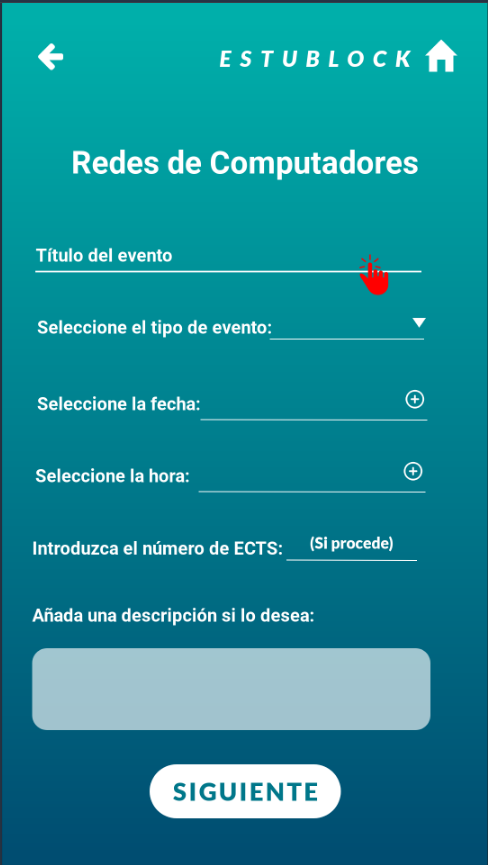
\includegraphics[width=0.5\linewidth]{figs/Desarrollo/Interfaz/marvel_crear_evento}
        \caption[Marvel Crear Evento]{Pantalla de creación de evento de marvelapp}
	\end{subfigure} 
	\begin{subfigure}[b]{0.4\linewidth}
		\centering
        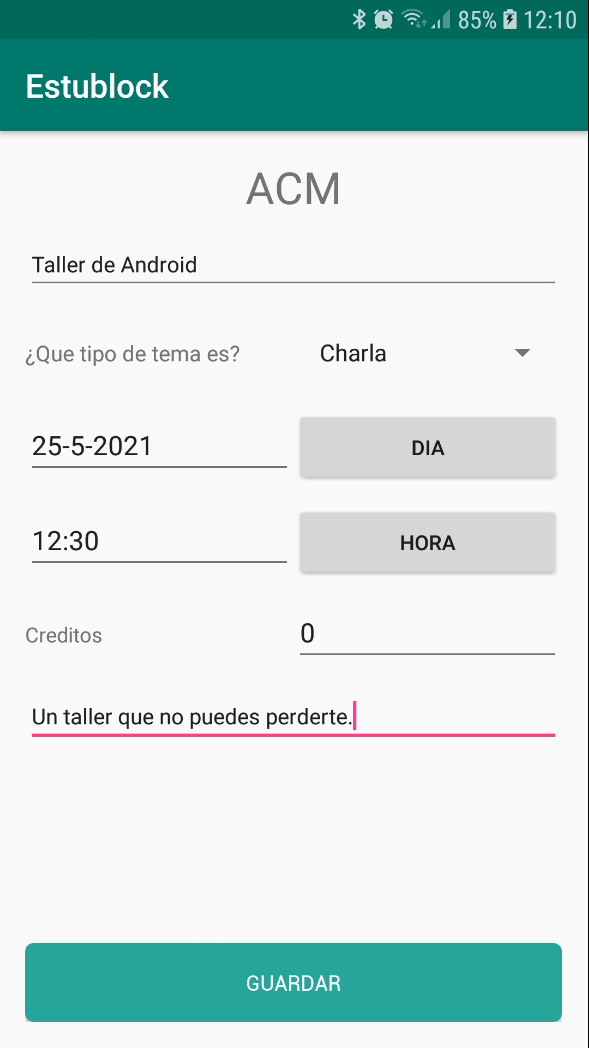
\includegraphics[width=0.5\linewidth]{figs/Desarrollo/Interfaz/estublock_crear_evento_completo.png}
        \caption[Estublock Crear Evento]{Pantalla de creación de evento de Estublock}
	\end{subfigure} 
	\caption[Pantalla de Crear Evento]{Pantalla de Crear Evento}
	\label{fig:pantalla_crear_evento}
\end{figure}

\begin{figure}[hbt]
	\centering
	\begin{subfigure}[b]{0.4\linewidth}
		\centering
        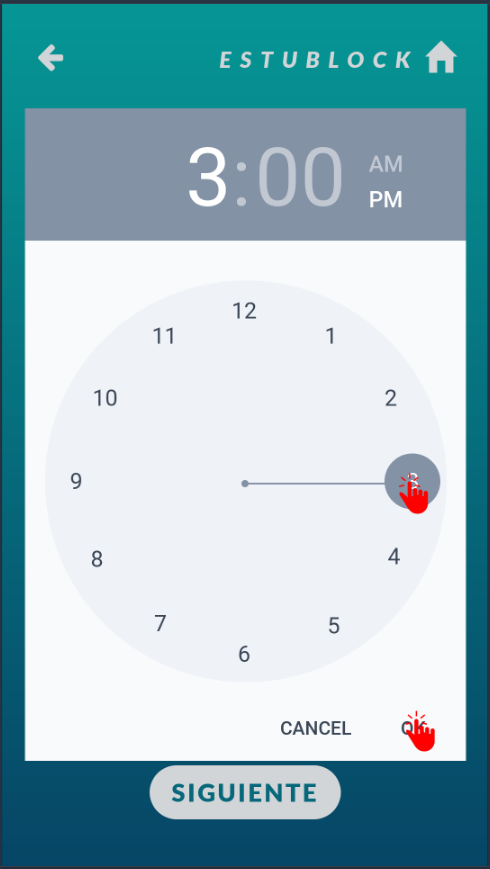
\includegraphics[width=0.5\linewidth]{figs/Desarrollo/Interfaz/marvel_crear_evento_hora}
        \caption[Marvel Hora]{Pantalla de hora de marvelapp}
	\end{subfigure} 
	\begin{subfigure}[b]{0.4\linewidth}
		\centering
        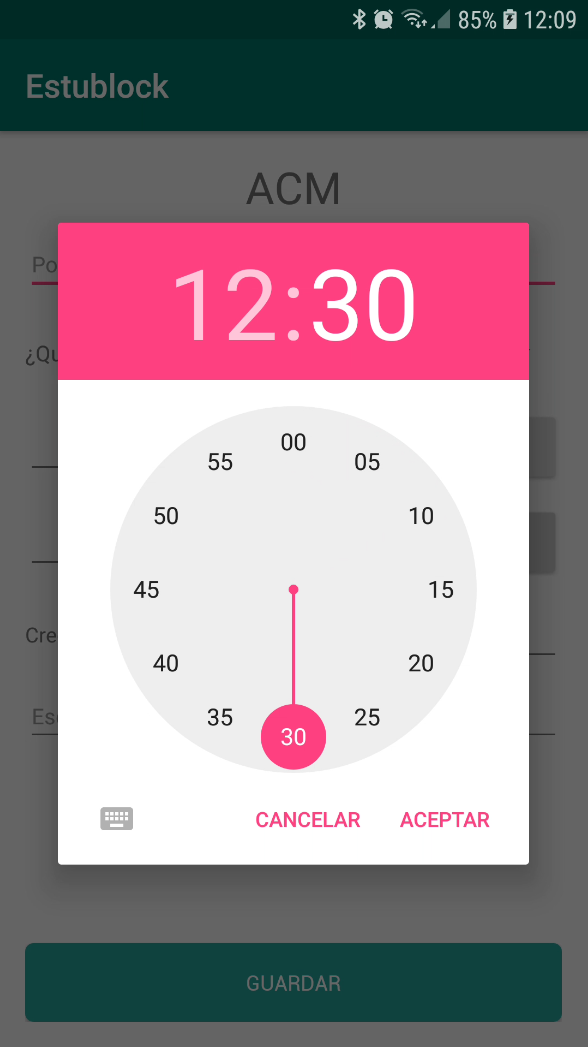
\includegraphics[width=0.5\linewidth]{figs/Desarrollo/Interfaz/estublock_crear_evento_hora}
        \caption[Estublock Hora]{Pantalla de hora de Estublock}
	\end{subfigure} 
	\caption[Pantalla de Hora]{Pantalla de Hora}
	\label{fig:pantalla_hora}
\end{figure}

\subsubsection{Pantalla de generar un QR}

Para llegar a esta pantalla, el usuario ha elegido previamente el botón \verb|Asistencia| así como seleccionar la asignatura y evento al que se quiere registrar. En la pantalla, aparece un gran QR que el profesor debe escanear. Esto es \textbf{muy importante}, es uno de los grandes cambios en la forma en la que se registra la asistencia. Al diseñar la aplicación ``Estublock'' en Marvelapp, se planteó que el profesor enseñaría el QR y los alumnos lo escanearían. Sin embargo ahora se hace al revés. Esta decisión se ha tomado, ya que quien tiene que firmar las transacciones a la red Blockchain es el profesor, para ello, tiene que ser él quien lea los datos de un alumno y firme con su wallet que ese alumno ha asistido al exámen. Luego, la pantalla ha quedado más sencilla, pero con mucho más espacio para él QR y así facilitar su escaneo. La pantalla del QR se puede ver a continuación \ref{fig:pantalla_qr}

\begin{figure}[hbt]
	\centering
	\begin{subfigure}[b]{0.4\linewidth}
		\centering
        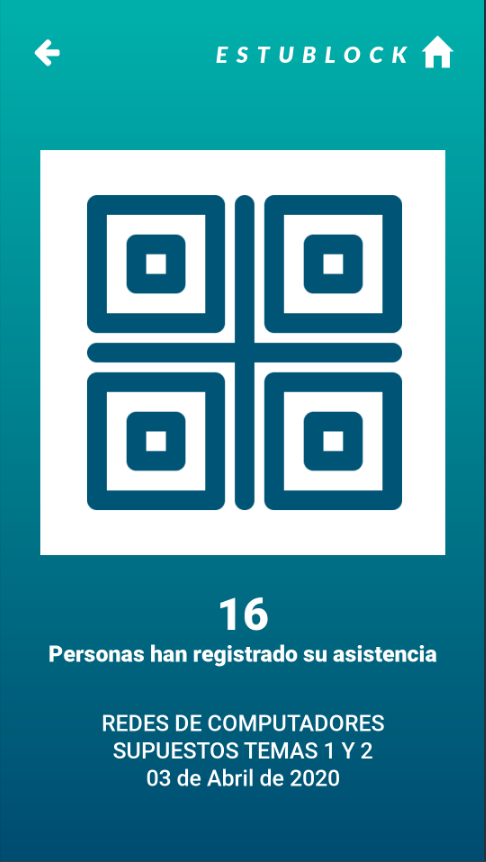
\includegraphics[width=0.5\linewidth]{figs/Desarrollo/Interfaz/marvel_QR}
        \caption[Marvel QR]{Pantalla de QR de marvelapp}
	\end{subfigure} 
	\begin{subfigure}[b]{0.4\linewidth}
		\centering
        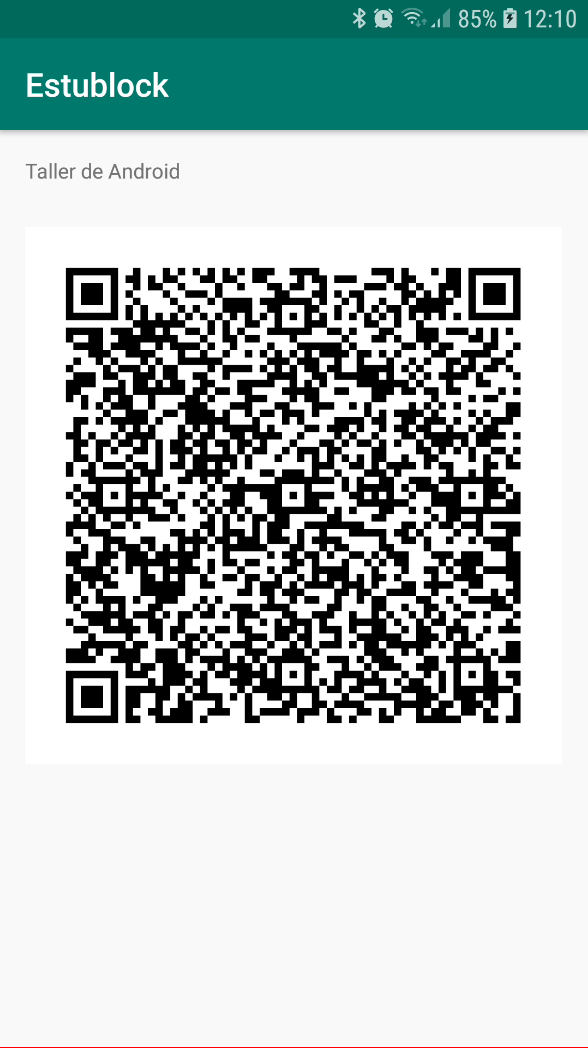
\includegraphics[width=0.5\linewidth]{figs/Desarrollo/Interfaz/estublock_QR}
        \caption[Estublock QR]{Pantalla de QR de Estublock}
	\end{subfigure} 
	\caption[Pantalla de QR]{Pantalla de QR}
	\label{fig:pantalla_qr}
\end{figure}

\subsubsection{Pantalla del Escanear un QR}

Esta pantalla es especial, pues llama a la actividad de la \textbf{cámara de fotos}. Como hemos visto anteriormente en el estado del arte, una aplicación puede llamar sin problemas a otra aplicación (siempre y cuando esta lo permita). En esta ocasión, se requiere de la cámara del usuario para escanear el QR. No todas las cámaras de los móviles escanean QRs de forma automática, pero esto no es un problema ya que la librería que se ha utilizado para programar esta actividad, se encarga de ello. El usuario entonces verá como se abre su cámara y al enfocar un QR, este se escanea automáticamente enviando a la red blockchain la asistencia. Una representación visual puede verse en \ref{fig:pantalla_escaneo_qr}

\begin{figure}[h!]
  \centering
  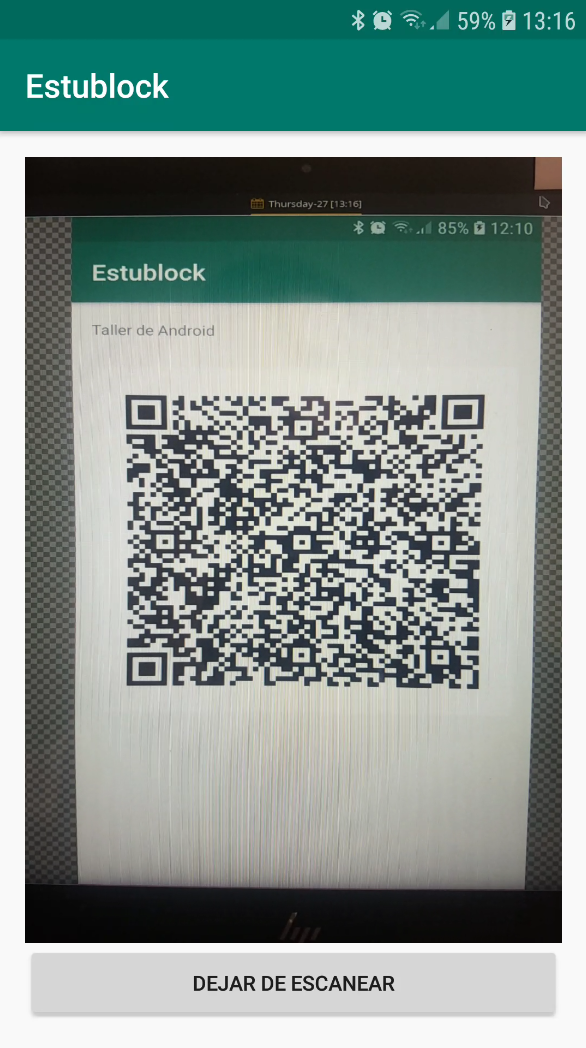
\includegraphics[width=0.3\linewidth]{figs/Desarrollo/Interfaz/estublock_escanear_qr}
  \caption[Pantalla de Escaneo de QR]{Pantalla de escaneo de QR Estublock}
  \label{fig:pantalla_escaneo_qr}
\end{figure}

% --------------------------------------------------
\subsection{Código XML}

Como ya hemos mencionado, las interfaces de usuario en Android se programan utilizando código XML. XML, del ingles \emph{Extensible Markup Language} es un metalenguaje que permite definir con un lenguaje de marcas información y datos. Es parecido a HTML, pero las etiquetas no estan predefinidas sino que puedes inventarte las que quieras. Permite crear estructuras con parámetros y atributos los cuales pueden utilizarse por ejemplo en internet para enviar datos a una API. En el caso de las aplicaciones móvil, el código XML se utiliza para diseñar las pantallas o \emph{layouts}, ya que XML es un lenguaje ligero y esto hace que las pantallas sean ligeras también. Es con el código XML con el que se definen las jerarquías que se mencionan en el apartado \hyperref[sec:GUI]{3.2.1}, por ejemplo, parte de la estructura de la pantalla \emph{crear un evento} puede verse en \ref{fig:xml_crear_evento} se han omitido los atributos para ahorrar espacio. 

\begin{figure}[h!]
  \centering
  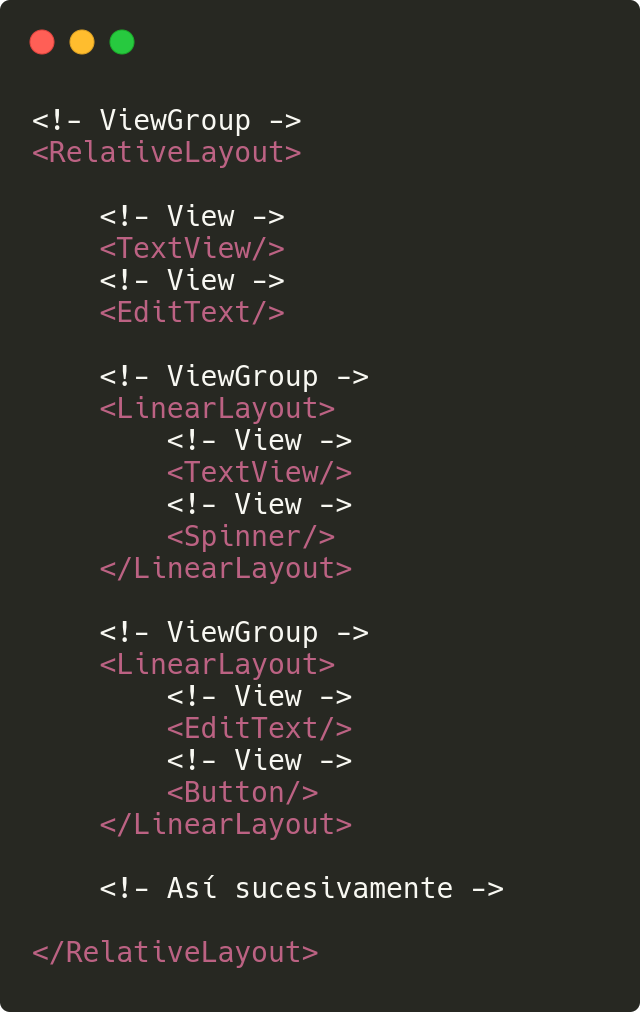
\includegraphics[width=0.95\linewidth]{figs/Desarrollo/Codigo/xml_jerarquia}
  \caption[XML Jerarquia]{Fragmento de la jerarquía XML de la pantalla crear evento}
  \label{fig:xml_crear_evento}
\end{figure}

Programar pantallas para Android sin ningún tipo de feedback, es decir, sin saber como esta quedando la pantalla, es muy difícil. Por eso, Android Studio, trae consigo una herramienta de gran utilidad, la que cual permite visualizar y editar el código sin tener que escribirlo por completo. Se puede por ejemplo crear un botón, y la herramienta de forma automática escribirá el código XML correspondiente, luego se puede cambiar el color del botón, y la herramienta se encargará de escribir el código XML correspondiente. Sin embargo, tras una actualización de Android Studio (actualización a la versión 4.2.0.24-1) el sistema de atributos dejó de funcionar, y hubo que añadir los atributos manualmente, esto supuso un tiempo extra a la hora de realizar las pantallas, y es una de las razones por las que las pantallas (excepto login y registro) han quedado visualmente más básicas. La herramienta de Android Studio puede encontrarse en la figura\ref{fig:herramienta_android}.

\begin{figure}[h!]
  \centering
  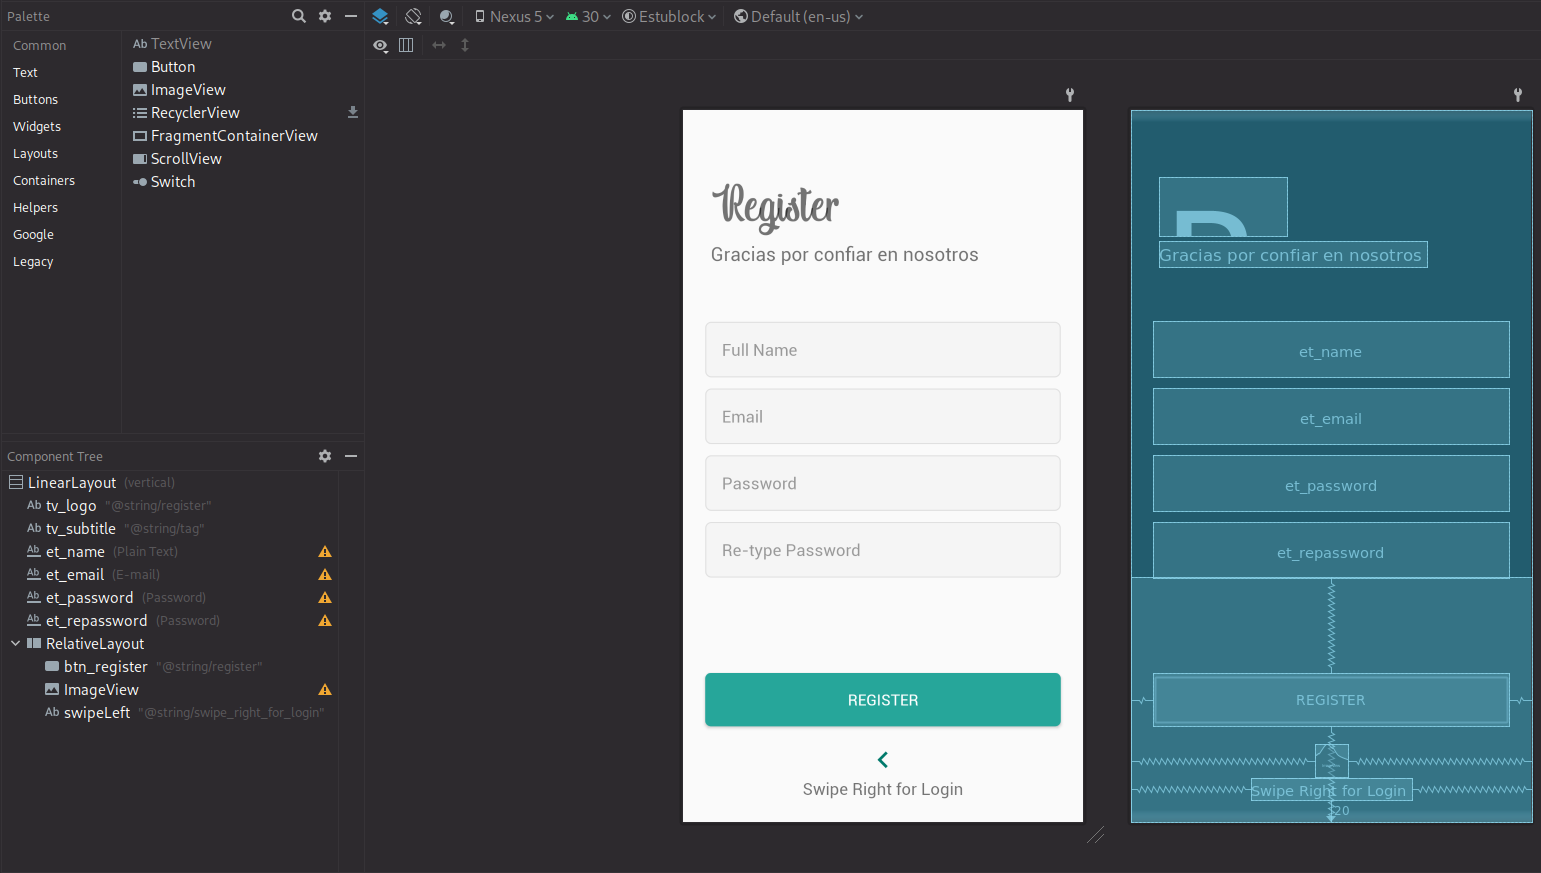
\includegraphics[width=0.95\linewidth]{figs/Desarrollo/XML/androidStudio}
  \caption[XML Herramienta Android Studio]{Herramienta de Android Studio para la edición de layouts (pantallas)}
  \label{fig:xml_crear_evento}
\end{figure}

XML no solo sirve para diseñar las pantallas, hasta ahora todo lo que hemos comentado se refería al esqueleto de una pantalla. Es decir, un botón arriba, un texto pegado abajo a la derecha\dots Pero con XML también se puede modificar la apariencia, color, forma, fuente de todos los elementos. Dentro de las carpetas de un proyecto Android, tenemos algunas carpetas en las que se guarda código XML que se utiliza posteriormente para darle un mejor diseño a un elemento. Por ejemplo, se puede crear un botón y asignarle un fondo con el atributo \verb|android:background| a este atributo se le añade como parámetro la ruta al archivo que contiene la información en XML sobre como queremos que se vea este botón. Por otro lado, hemos mencionado también las fuentes, los archivos que modifican las fuentes son de tipo \emph{TrueType Font} y definen la fuente de las letras. Por ejemplo, si creamos un campo de texto \verb|TextView| podemos ponerle una fuente especifica con el atributo \verb|android:fontFamily|. Básicamente, somos libres de modificar con total control cada aspecto que se quiera de las pantallas. \\

Por último, haremos mención de una carpeta muy importante llamada \textbf{values} en la que se guardan parámetros para definir los colores, las dimensiones de la pantalla, los distintos temas disponibles y un archivo llamado \textbf{strings} el cual guarda todo el texto estático que se quiere añadir a las pantallas. Este archivo existe, para facilitar el migrado de la aplicación a otros idiomas. Por ejemplo, en vez de escribir en un \verb|TextView| una palabra en español, se le asignará un identificador dentro del archivo \emph{strings}, de modo que si alguna vez tenemos varios idiomas disponibles, se puede tener con el mismo identificador la palabra en varios idiomas, y será tan sencillo como decirle a Android que utilice un archivo \emph{strings} u otro, de modo que las pantallas no hay que modificarlas nunca si se quiere cambiar de idioma. Lo mismo aplica a los colores, temas (si queremos un tema oscuro, no hay que cambiar las pantallas sino que se cambian los colores del archivo de temas y el archivo de colores)\dots Básicamente, aportan flexibilidad y escalabilidad en la aplicación para poder modificarla con más seguridad y rapidez. 




% --------------------------------------------------
\section{Código} \label{sec:Codigo}

Las aplicaciones Android pueden ser programadas principalmente en dos lenguajes de programación, \textbf{Java} y \textbf{Kotlin}. En el presente, la inmensa mayoría de aplicaciones han sido desarrolladas con Java, sin embargo Kotlin es promete ser el futuro. Actualmente sigue siendo un lenguaje muy secundario (aunque se puede hacer todo lo que se puede hacer con Java y esta muy bien documentado). Según google trends\ref{fig:java_vs_kotlin}, Kotlin esta lejos de quitarle el puesto a Java aunque los nuevos desarrolladores de aplicaciones Android muestran más interés por Kotlin por su comodidad, falta de verbosidad y ``limpieza'' (es decir, con menos líneas de código haces lo mismo que Java). 

\begin{figure}[h!]
  \centering
  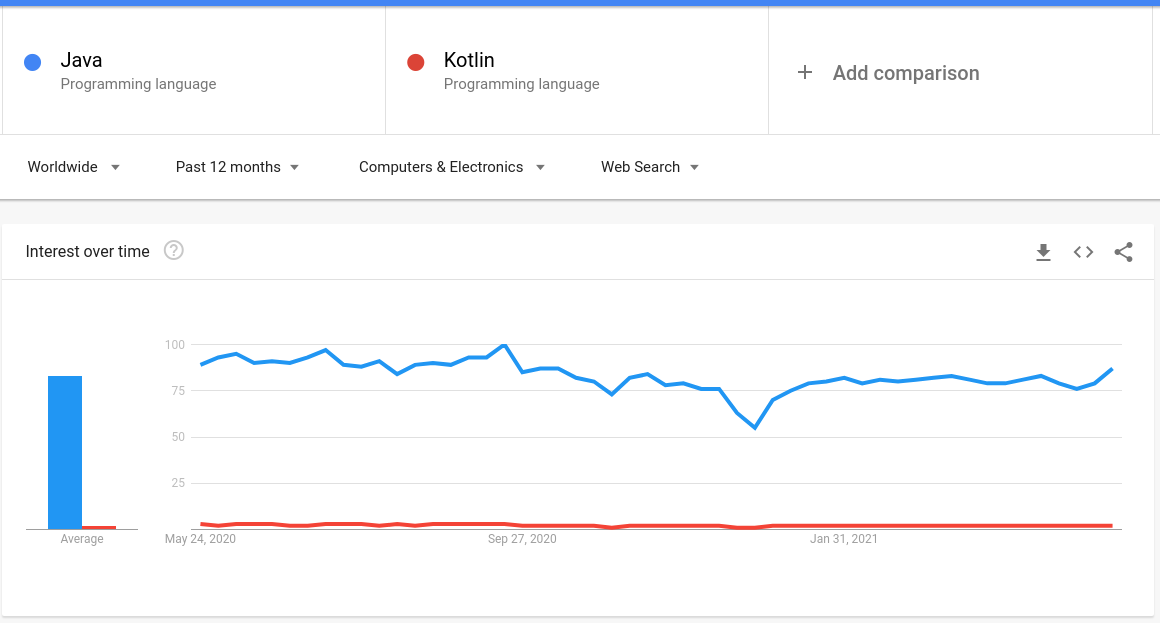
\includegraphics[width=0.6\linewidth]{figs/Desarrollo/Popularidad}
  \caption[Java vs Kotlin]{Comparación de Google Trends entre Java y kotlin}
  \label{fig:java_vs_kotlin}
\end{figure}

Por lo tanto, aunque Kotlin promete mucho, la aplicación Estublock se ha desarrollado en el lenguaje Java para tener una mayor cantidad de documentación y de comunidad disponible. Con comunidad, nos referimos a las personas en el planeta que saben de programación Android con Java y que a lo largo de los años han respondido y contribuido en Internet, dando soluciones a problemas, documentación y contando sus trucos profesionales. De todos modos, se puede migrar con mucha facilidad a Kotlin puesto que AndroidStudio permite migrar automáticamente de Java a Kotlin. Lo único que se necesita para facilitar este proceso es añadir ``anotaciones de java'' que especifiquen las características de algunas variables o funciones para facilitar a AndroidStudio el reconocimiento de las variables. Un ejemplo puede encontrarse a continuación donde se puede ver que se especifica que la variable no puede ser nula con \emph{@NonNull}.

\begin{lstlisting}[language=Java,float=ht,caption={[Java] Ejemplo de ``anotación de java'' de variables para facilitar el salto a Kotlin},label=lst:java_etiquetas]
public void sendSignedTransaction(@NonNull String signedMessage){
  // Código
}
\end{lstlisting}

% --------------------------------------------------
\subsection{Código Java}

Todo el código de la aplicación esta disponible en mi repositorio de github\cite{forgis98}. Vamos a tratar de resumir el trabajo realizado, pues gran parte de este TFG esta reflejado en la aplicación móvil que se ha desarrollado. \\

\subsubsection{Archivos del Proyecto}

% Manifest XML
% Gradle
% Estructura de Estublock
% Estructura del SDK

Un proyecto en Android Studio dispone de un gran conjunto de carpetas y archivos que hacen funcionar a la aplicación entera. En el caso de ``Estublock'' vamos a mencionar los que son de gran importancia. Empezando por \textbf{AndroidManifest.xml}, todos los proyectos Android deben tener un archivo con este nombre en la raíz del proyecto. Este archivo, describe información esencial de la aplicación para las herramientas de creación de Android y para el sistema operativo. Entre otras cosas, el archivo declara el nombre del paquete que contiene la aplicación, los componentes de la aplicación (actividades, servicios\dots), los permisos de los que requiere la aplicación como permiso a la cámara o a internet como en el caso de ``Estublock''. Si se usa Android Studio, este archivo se creará automáticamente pero para añadir permisos ha de hacerse manualmente. En el proyecto ``Estublock'' se han añadido a este archivo los permisos de acceso a \textbf{Internet}, escritura de \textbf{datos en memoria} y a la \textbf{cámara} del dispositivo. \\

Por otro lado, toda una carpeta de gran importancia en el proyecto es la carpeta de \textbf{Gradle}. Gradle es un paquete de herramientas de compilación avanzadas, que permite automatizar y administrar el proceso de compilación. Al ser una herramienta de compilación, trae consigo un conjunto de carpetas y archivos que utiliza para gestionar el proyecto, en concreto esta el archivo \textbf{build.gradle} en el que se escriben las dependencias del proyecto para poder utilizar librerías no incluidas por defecto en java o Android. A la hora de desarrollar la aplicación, se han añadido varias librería que se verán en mejor detalle en \hyperref[sec:librerias]{Librerías} como \textbf{okhttp, bcrypt, web3j}\dots \\

La estructura de carpetas del SDK, es muy parecida a la de ``Estublock'' con la principal diferencia de que no tiene ninguna carpeta de interfaz (no tiene carpetas de colores, temas, strings, layouts\dots). Sin embargo tiene su propio archivo \emph{build.gradle} y su propio archivo \emph{AndroidManifest.xml}. Puesto que no tienen grandes diferencias, mostramos solo la estructura de la carpeta que contiene el proyecto ``Estublock'' pues tiene más contenido que el SDK \ref{fig:jerarquia_estublock} \\

\begin{figure}[h!]
  \centering
  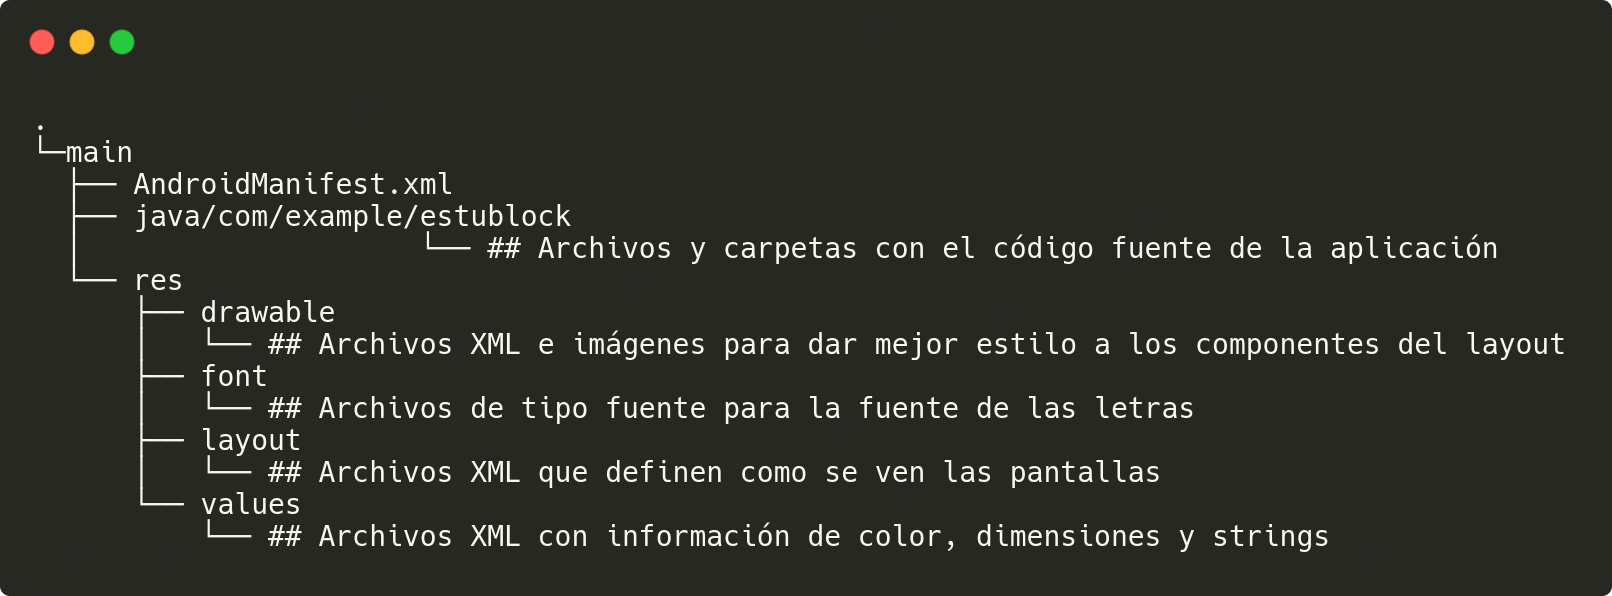
\includegraphics[width=0.6\linewidth]{figs/Desarrollo/JerarquiaCarpetas}
  \caption[Jerarquia Estublock]{Jerarquia de carpetas del proyecto Estublock}
  \label{fig:jerarquia_estublock}
\end{figure}

Por último, al ejecutar la aplicación en el dispositivo móvil por primera vez y registrar a un usuario, se crea en el directorio de carpetas del usuario dos archivos nuevos. Uno de ellos es el \hyperref[sec:wallet]{wallet} del cual hablaremos más adelantes. Y el otro es una carpeta con un archivo en el que guardar datos en forma de un par \{claves $->$ valor\}. Este carpeta se llama \textbf{shared preferences}. En el caso de la aplicación, se utiliza para guardar el directorio en el que se ha guardado el wallet.

\subsubsection{Librerías utilizadas} \label{sec:librerias}

Se han utilizado 8 librerías extras (a parte de las que incluye por defecto android al iniciar el proyecto). \emph{web3j} se mencionará en el apartado del \hyperref[sec:SDK]{SDK} y \emph{play-services-vision} es necesaria para \emph{ZXing} pero no se ha usado directamente. Queda entonces: \\
\begin{enumerate}
\item \textbf{Volley: } Volley es una biblioteca HTTP que facilita y agiliza el uso de redes en apps para Android. Permite programación automática de solicitudes de res, varias conexiones de red simultáneas, almacenamiento de respuestas en cache\dots Se ha utilizado esta librería para todas las llamadas excepto la llamadas \emph{DELETE} ya que me daba problemas. Algo muy interesante de Volley es que las llamadas son asíncronas, es decir, se ejecutan separadas del hilo principal no bloqueándolo y una vez se recibe la respuesta de la llamada se puede recuperar la información en un callback. Un ejemplo de llamada POST puede verse en \ref{fig:post_volley} \\

% \begin{lstlisting}[language=Java,float=ht,caption={[Java] Ejemplo de llamada POST con Volley.},label=lst:volley]
% JsonObjectRequest jsonObjectRequest = new JsonObjectRequest(Request.Method.POST,
%     (URL), parametrosJSON,
%     new Response.Listener<JSONObject>() {
%       @Override
%       public void onResponse(JSONObject response) {
%         // Hacer algo con respuesta correcta.
%       }
%     }, new Response.ErrorListener() {
%   @Override
%   public void onErrorResponse(VolleyError error) {
%     // Hacer algo con respuesta error.
%   }
% });
% \end{lstlisting}

\begin{figure}[h!]
  \centering
  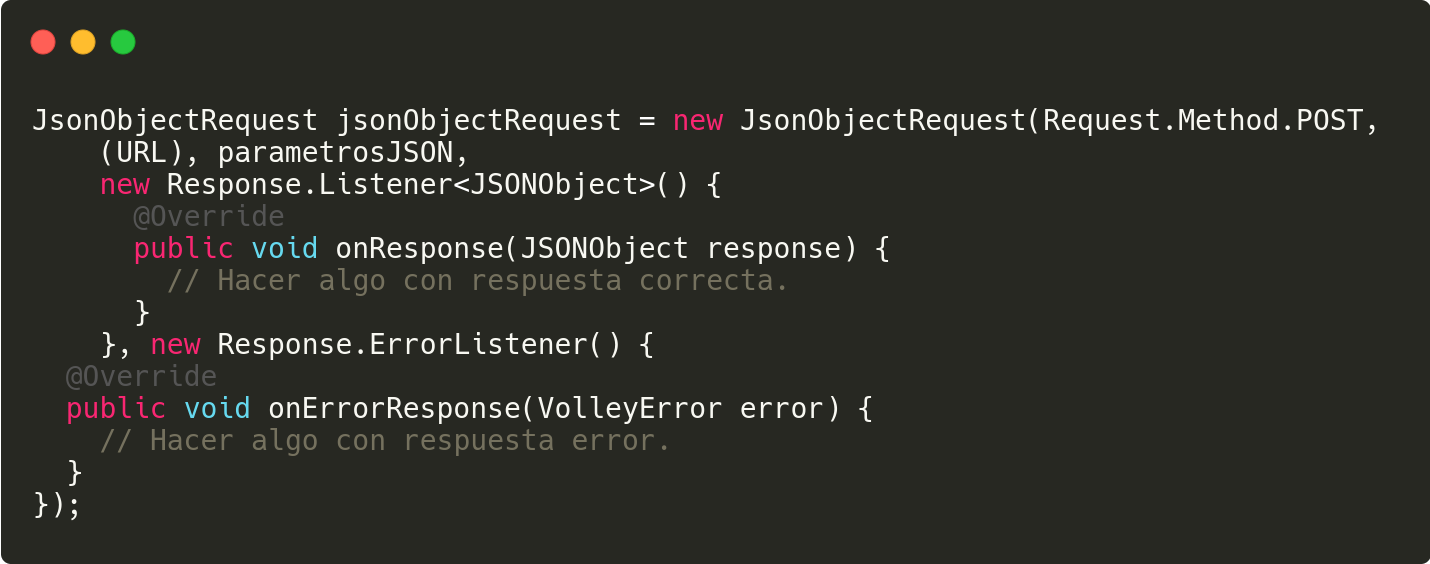
\includegraphics[width=0.8\linewidth]{figs/Desarrollo/Codigo/POST_Volley}
  \caption[Llamada POST con Volley]{Ejemplo de llamada POST con Volley}
  \label{fig:post_volley}
\end{figure}

Para solventar el problema con la llamada DELETE se ha usado la librería Okhttp.

\item \textbf{Okhttp: } Esta librería cumple la misma función que Volley, permitiendo conexiones HTTP\dots Sin embargo, Volley es asíncrono. Okhttp no lo es, ``obligando'' al programador a hacer las llamadas dentro de un hilo de ejecución nuevo. Un ejemplo se provee en la figura \ref{delete_okhttp}

% \begin{lstlisting}[language=Java,float=ht,caption={[Java] Ejemplo de llamada DELETE con OkHttp.},label=lst:okhttp]
% new Thread(new Runnable() {
%   @Override
%   public void run() {
%     try{
%       // Hacer cosas dentro del Thread
% 
%       okhttp3.RequestBody body = okhttp3.RequestBody.create(
%         paramsJSON.toString(), 
%         MediaType.parse("application/json; charset=utf-8")
%       );
% 
%       okhttp3.Request request = new okhttp3.Request.Builder()
%         .url(URL)
%         .delete(body)
%         .build();
%       okhttp3.Response response = client.newCall(request).execute();
% 
%     } catch(Exception e){
%       // Hacer cosas en caso de error.
%     }
%   }
% }).start();
% \end{lstlisting}

\begin{figure}[h!]
  \centering
  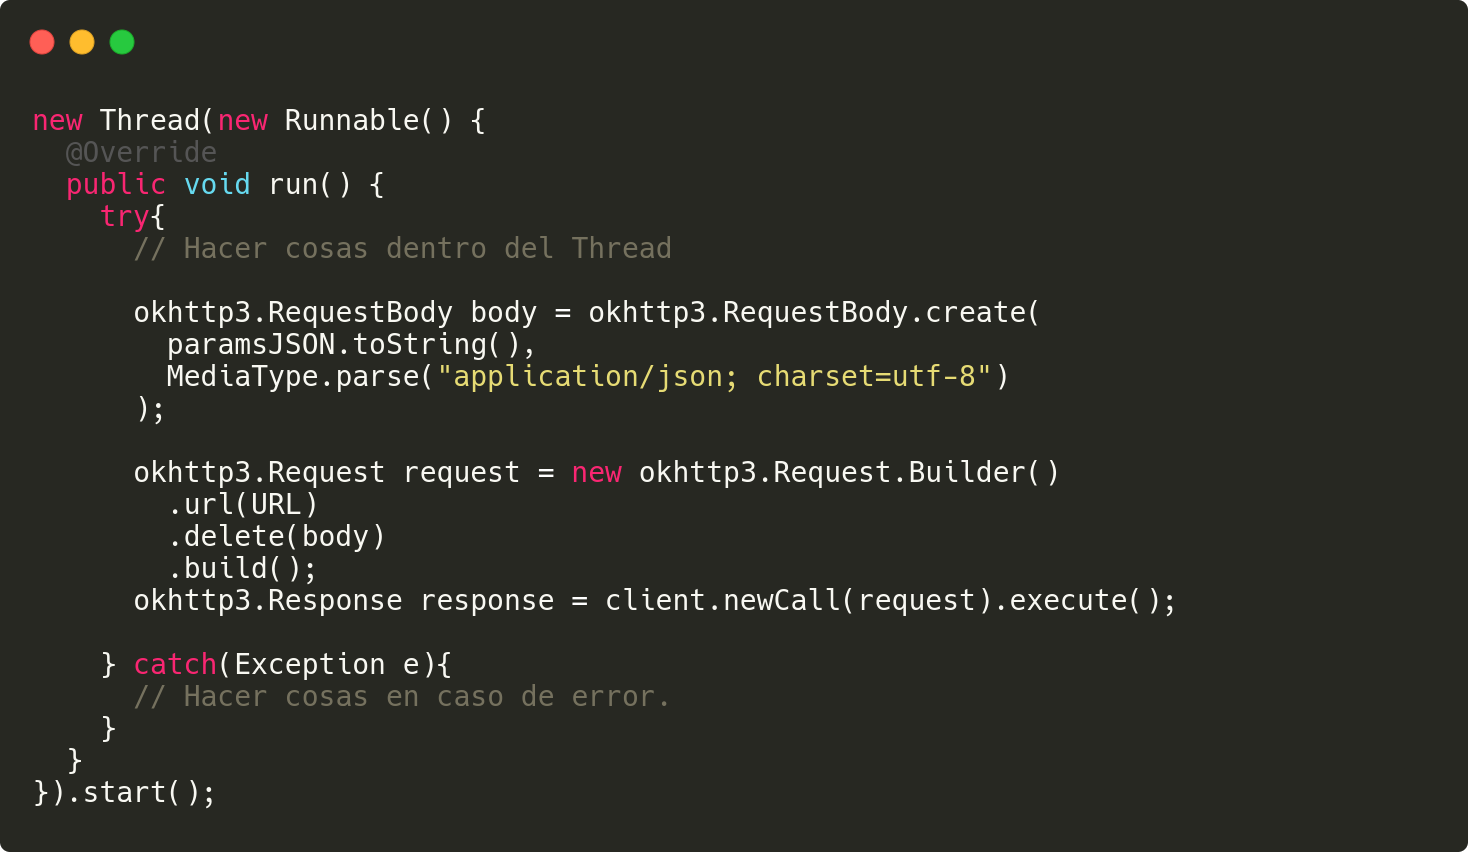
\includegraphics[width=0.8\linewidth]{figs/Desarrollo/Codigo/okhttp_ejemplo}
  \caption[Llamada DELETE con Okhttp]{Ejemplo de llamada DELETE con OkHttp}
  \label{fig:delete_okhttp}
\end{figure}

\item \textbf{Bcrypt: } Es una implementación del algoritmo de hash de contraseñas Blowfish. Básicamente permite cifrar contraseñas para poder guardarlas de forma segura en una base de datos. Con esta librería se cifra la contraseña del usuario que luego se manda a la API para que la guarde en la base de datos como se puede ver en \ref{fig:bcrypt}

% \begin{lstlisting}[language=Java,float=ht,caption={[Java] Ejemplo de cifrado de la contraseña de un usuario.},label=lst:okhttp]
% protected String hashPassword(String password){
%   return BCrypt.withDefaults().hashToString(10, password.toCharArray());
% }
% \end{lstlisting}

\begin{figure}[h!]
  \centering
  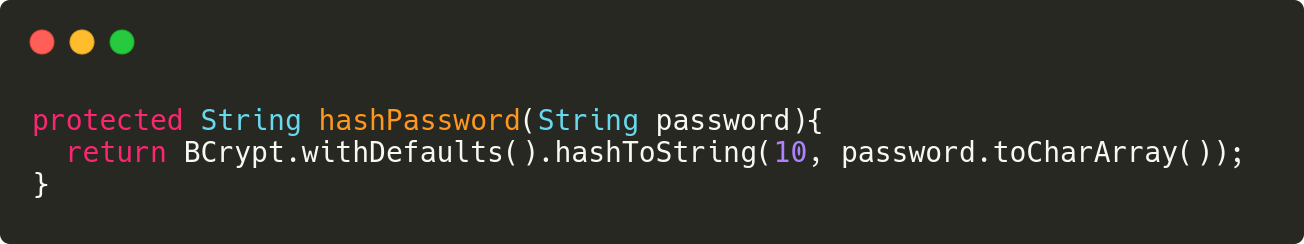
\includegraphics[width=0.8\linewidth]{figs/Desarrollo/Codigo/bcrypt}
  \caption[Ejemplo de cifrado de contraseñas]{Ejemplo de cifrado de la contraseña del usuario}
  \label{fig:bcrypt}
\end{figure}


\item \textbf{QRGenerator: } Librería para generar códigos QR tanto 1D (códigos de barra) como 2D (QR tradicional) con diferentes formatos. Vease \ref{fig:generador_qr}

% \begin{lstlisting}[language=Java,float=ht,caption={[Java] Ejemplo de Código QR},label=lst:okhttp]
% WindowManager manager = (WindowManager) getSystemService(WINDOW_SERVICE);
% Display display = manager.getDefaultDisplay();
% Point point = new Point();
% display.getSize(point);
% 
% qrgEncoder = new QRGEncoder(evento.toString(), null, QRGContents.Type.TEXT, Math.min(point.x, point.y));
% bitmap = qrgEncoder.getBitmap();
% // qr es el identificador de la interfaz de usuario para poner el QR
% qr.setImageBitmap(bitmap);
% \end{lstlisting}

\begin{figure}[h!]
  \centering
  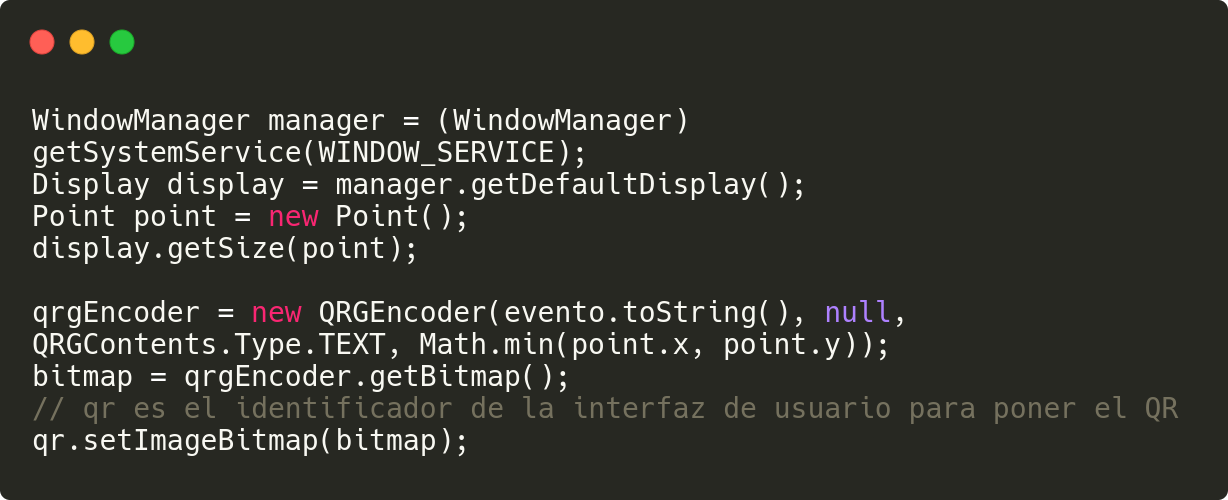
\includegraphics[width=0.8\linewidth]{figs/Desarrollo/Codigo/generador_QR}
  \caption[Ejemplo básico de generar QR]{Ejemplo básico de código de generar QR}
  \label{fig:generador_qr}
\end{figure}

\item \textbf{ZXing: } Esta librería permite generar códigos QR, pero más importante y la razón por la que se ha usado, permite escanear códigos QR. Para generar QR se utilizó la librería anterior puesto que su uso es más fácil de utilizar que ZXing para Android. El código en este caso es bastante más largo por lo que se ha incluido en el \hyperref[cap:Anexo]{Anexo} en concreto en \ref{fig:escaneandoQRs}.

\end{enumerate}

\subsubsection{Archivo GlobalState}

Todos los archivos de código fuente son muy importantes, pues engloban toda la funcionalidad de la aplicación. A la hora de desarrollar aplicaciones, en ocasiones hay que tener en cuenta la información que se quiere guardar sobre el usuario que ha hecho login temporalmente (en ejecución). Una forma de pasar información de una pantalla a otra para mantener por ejemplo el correo de un usuario y poder usarlo en otras pantallas sin tener que volver a pedírselo es utilizando los \emph{Intents}. Un Intent es una descripción abstracta de una operación a realizar, puede utilizarse para lanzar otras actividades y junto al lanzamiento pasar como parámetros valores como se puede ver en \ref{fig:intents} \\

\begin{figure}[h!]
  \centering
  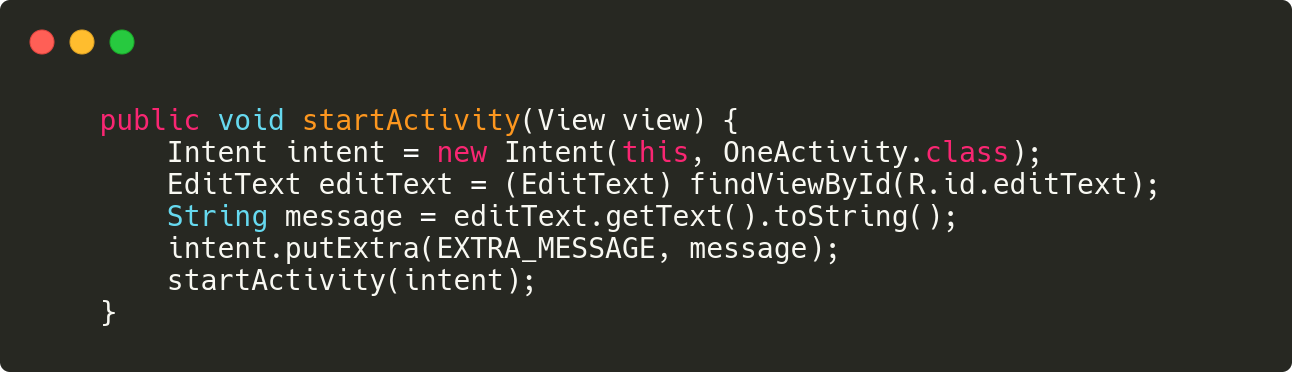
\includegraphics[width=0.8\linewidth]{figs/Desarrollo/Codigo/intents}
  \caption[Ejemplo de Intent en Android]{Ejemplo de Intent en Android}
  \label{fig:intents}
\end{figure}

Sin embargo esto trae una desventaja, siempre que se pase de una a otra pantalla hay que añadir los datos que se quieren guardar para no perderlos, esto puede hacer que si quieres un dato en muchas pantallas, acabes acumulando datos, y hace que el código sea menos legible. Por lo tanto, se tomó la decisión de crear un archivo especial llamado \textbf{GlobalState.java}. Este archivo no tiene una actividad (pantalla) correspondiente, pues su único propósito es el de guardar el estado de algunos datos para evitar pedírselos nuevamente al usuario. Datos como el correo, nombre, directorio donde esta el wallet\dots Pero también se ha aprovechado para guardar las URL de las APIs, nodo de la blockchain\dots El código de este archivo esta disponible en el Anexo ref{fig:gs}



% ##################################################
% ##################################################
\section{SDK} \label{sec:SDK}

Un \emph{Kit de Desarrollo Software} o SDK (Software Development Kit) es generalmente un conjunto de herramientas de desarrollo de software que permiten a otros desarrolladores crear aplicaciones de forma más cómoda. Un buen ejemplo de SDK que se ha utilizado en este proyecto es la familia de SDKs de Android. Junto con AndroidStudio, se instalan múltiples SDKs que permiten al programador escribir código, recuperar componentes de las pantallas, hacer llamadas a paquetes, importar paquetes, detectar errores\dots Todo de forma automática haciendo que la programación sea mucho más fácil. \\

El SDK es entonces un conjunto de métodos los cuales pueden hacer llamadas a una API, llamadas al propio sistema operativo, llamadas a otras librería o SDKs\dots En el caso del SDK desarrollado para este TFG, su principal función es la de hacer llamadas a una red blockchain y la de hacer llamadas al sistema de archivos del dispositivo para guardar la cartera virtual del usuario. 

% --------------------------------------------------
\subsection{Diseño del SDK}

El SDK dispone de 3 archivos separados del proyecto Estublock. Se han creado como librería desde AndroidStudio para poder compartirla después públicamente y que otros programadores puedan utilizarla. Se ha dividido en 3 archivos para tratar de mantener una coherencia entre las funcionalidades que ofrece el SDK. Uno de los archivos se encarga únicamente de gestionar las transacciones, otro archivo se encarga únicamente de gestionar el wallet del usuario, y por último un archivo que se encarga de gestionar los callbacks de las llamadas a la red blockchain, pues estas se ejecutan de manera asíncrona. \\

Por otro lado, con respecto al diseño de los métodos, se ha optado por tratar de programarlos de la forma más genérica posible para que puedan aplicarse en una amplia variedad de situaciones, además se han sobrecargado los métodos (más adelante veremos que significa sobrecargar métodos) para que se puedan utilizar distintos tipos de variables en las funciones sin problema. 

% --------------------------------------------------
\subsection{Comunicación con la Red Blockchain}

En el archivo \emph{TransactionsHelper.java} se encuentra importada la librería de \emph{web3j} y se encuentra también el código que firma y envía las transacciones. Web3j es una biblioteca de Java y Android que permite trabajar con smart contracts e integrarse con clientes o nodos en la red de \emph{Ethereum}. Esto permite trabajar con la red de Ethereum sin necesidad de implementar el código de integración para la plataforma. Implementa la API de cliente JSON-RPC de Ethereum sobre HTTP, soporta carteras virtuales, firmado de transacciones\dots \\

El uso de \emph{TransactionsHelper} es sencillo, primero se crea el objeto pasándole como parámetro la URL del nodo de la red blockchain al que vamos a conectarnos \ref{fig:transH}
% \begin{lstlisting}[language=Java,float=ht,caption={[Java] Constructor de TransactionsHelper},label=lst:constructor]
% // Constructor
% public TransactionsHelper(@NonNull String blockchainURL){
%   web3j = Web3j.build(new HttpService(blockchainURL));
% }
% // Llamada 
% TransactionsHelper txHelp = new TransactionsHelper(URL);
% \end{lstlisting}

\begin{figure}[h!]
  \centering
  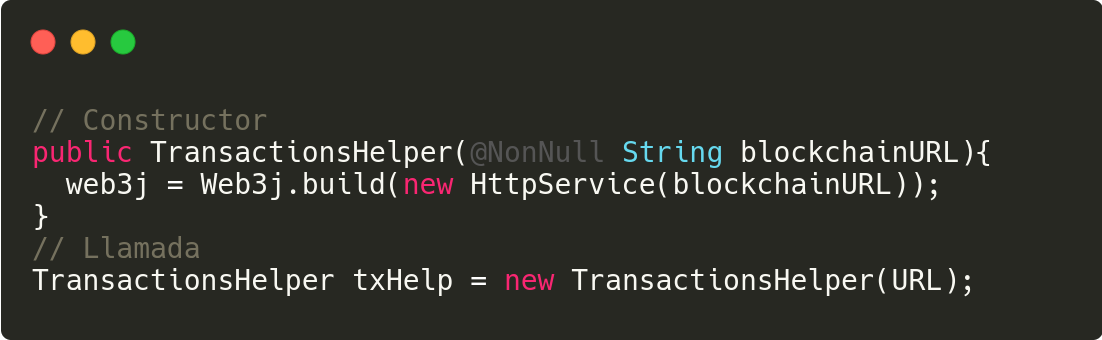
\includegraphics[width=0.8\linewidth]{figs/Desarrollo/SDK/transHelper_constructor}
  \caption[Constructor de TransactionsHelper]{Constructor de TransactionsHelper}
  \label{fig:transH}
\end{figure}

Una vez creado el objeto se puede llamar al resto de funciones, entre las que están \verb|signTransaction(...)| que recibe seis argumentos entre otros las credenciales de la cartera virtual, el destino de la transacción (el smart contract) y un \emph{listener} para recuperar la respuesta de la transacción. Recordemos, no se pueden hacer operaciones pesadas en el hilo principal de Android por lo que hay que hacerlo o en un hilo a parte. Otra función importante es \verb|sendSignedTransaction(...)| la cual recibe dos parámetros, la transacción firmada y un \emph{listener}. Ambas funciones están ``sobrecargadas'' (sobrecarga es la capacidad de un lenguaje de programación, que permite nombrar con el mismo identificador diferentes variables u operaciones), la razón de esta sobrecarga es permitir pasar los parámetro de múltples maneras. Por ejemplo, los datos de la transacción se pueden pasar como JSON, como String, como HashMap\dots y gracias a la sobrecarga podemos ponerle el mismo nombre a la función. A grandes rasgos un pequeño ejemplo de código puede verse en \ref{fig:firmEnv}

% \begin{lstlisting}[language=Java,float=ht,caption={[Java] Firmar y Enviar transacciones.},label=lst:transactionHelper]
% // Se crea y firma la transacción
% EthGetTransactionCount ethGetTransactionCount = null;
% ethGetTransactionCount = web3j.ethGetTransactionCount(credentials.getAddress(), DefaultBlockParameterName.LATEST).send();
% BigInteger nonce = ethGetTransactionCount.getTransactionCount();
% RawTransaction rawTransaction = RawTransaction.createTransaction(parametrosJSON);
% byte [] signedTx = TransactionEncoder.signMessage(rawTransaction, credentials)
% signedMessage = Numeric.toHexString(signedTx);
% 
% // Se envía la transacción
% EthSendTransaction ethSendTransaction = web3j.ethSendRawTransaction(signedMessage).send();
% \end{lstlisting}

\begin{figure}[h!]
  \centering
  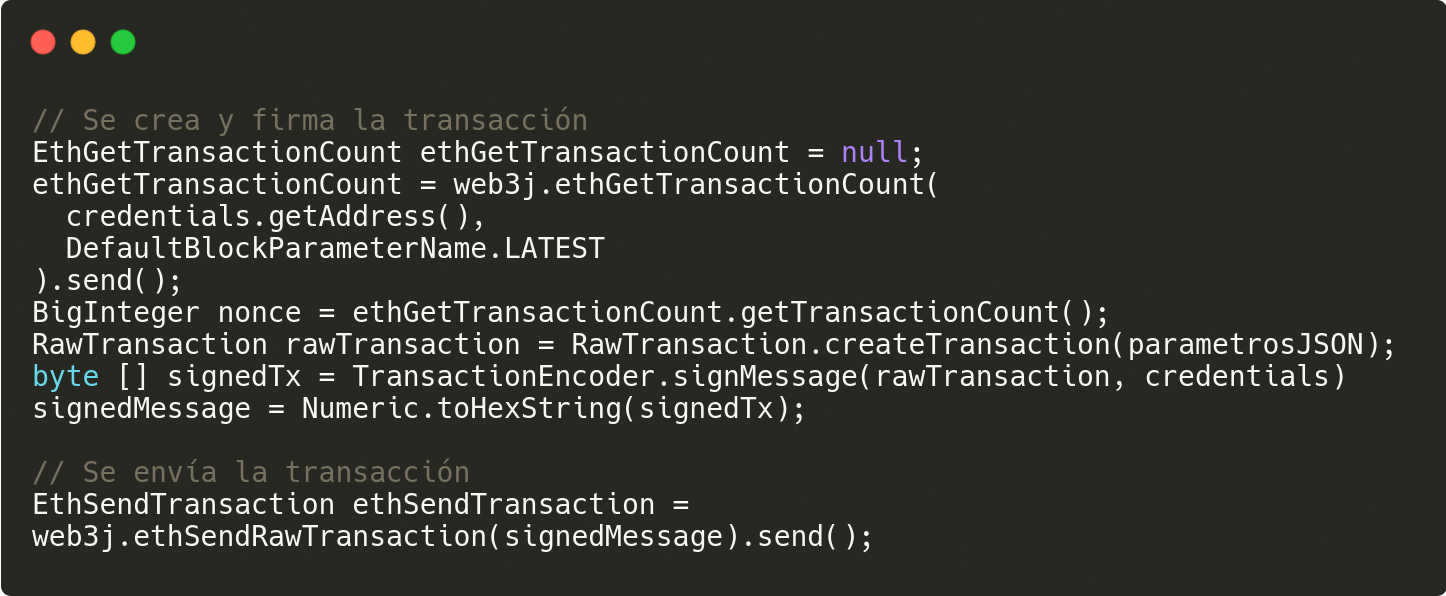
\includegraphics[width=0.8\linewidth]{figs/Desarrollo/SDK/firm_env_trans}
  \caption[Firmado y enviado de una transacción]{Firmado y enviado de una transacción}
  \label{fig:firmEnv}
\end{figure}



% --------------------------------------------------
\subsection{Comunicación con el Dispositivo}

Para facilitar la generación de credenciales, cartera virtual, guardar en la carpeta ``Shared Preferences'' de Android todos los datos necesarios para la comunicación con la red blockchain\dots Tenemos el archivo \emph{WalletHelper.java}. En él además de la librería web3j, tenemos algunas funcionalidades de Seguridad de Java para modificar el proveedor de seguridad, y permitir que salten errores por algoritmos o parámetros erróneos. \\

En este archivo tenemos entonces un constructor, el cual modifica el proveedor de seguridad a causa de un error con el algoritmo ``Elliptic Curve Digital Signature Algorithm''(ECDSA)\cite{ecdsa} para el proveedor BC\cite{bc}. Más información sobre el error se puede encontrar en el repositorio de web3j en la \href{https://github.com/web3j/web3j/issues/915}{issue\_915}. Básicamente lo que hace el código es modificar el proveedor.

\begin{lstlisting}[language=Java,float=ht,caption={[Java] Modificación de proveedor de seguridad},label=lst:transactionHelper]
final Provider provider = Security.getProvider(BouncyCastleProvider.PROVIDER_NAME);
if(provider != null || !provider.getClass().equals(BouncyCastleProvider.class)){
  Security.removeProvider(BouncyCastleProvider.PROVIDER_NAME);
  Security.insertProviderAt(new BouncyCastleProvider(), 1);
}
\end{lstlisting}

Luego, el programador dispone de varias funciones para crear una nueva cartera virtual con \verb|createNewWallet(...)| que acepta dos parámetros, siendo estos una contraseña y luego el lugar en el que se quiere guardar la cartera creada. Al igual que antes, esta función esta sobrecargada permitiendo pasar la localización como objeto String o como objeto File. Y permite también recuperar el \emph{address} del usuario o todas las credenciales. 

\begin{lstlisting}[language=Java,float=ht,caption={[Java] Creacion de wallet y recuperación del address},label=lst:transactionHelper]
WalletUtils.generateLightNewWalletFile(password, new File(keyStoreDirectory));

Credentials credentials = WalletUtils.loadCredentials(password, keyStoreDirectory);
String address = credentials.getAddress();
\end{lstlisting}

Como hemos mencionado anteriormente en este archivo se incluye también el guardado de los datos en él dispositivo móvil, aunque la función de web3j \verb|WalletUtils.generateLightNewWalletFile()| guarda los datos en el móvil. Para permitir que un usuario tenga varias carteras, se utiliza el \emph{SharedPreferences} para enlazar al usuario con su wallet. Para ello tenemos la función \verb|saveInPreferences(...)| la cual recibe cuatro parámetros entre ellos el lugar donde guardarlo, y los datos a guardar. Y luego tenemos otro método \verb|getFromPreferences(...)| para recuperar los datos. 

\begin{lstlisting}[language=Java,float=ht,caption={[Java] Guardado y recuperación de dátos en SharedPreferences},label=lst:transactionHelper]
// Guardamos los datos
SharedPreferences sharedPreferences = activity.getSharedPreferences(prefsName, Context.MODE_PRIVATE);
SharedPreferences.Editor editor = sharedPreferences.edit();
editor.putString(id, walletDirectory);
editor.apply();

// Devolvemos el dato con identificador id
return  sharedPreferences.getString(id, null);
\end{lstlisting}

% --------------------------------------------------
\subsection{``Callback Listener''}

Como las llamadas a la red blockchain son pesadas, han sido implementadas con threads: ``\verb|new Threads( new Runnable(){...} )|''. Como el código no espera a la respuesta del thread, he implementado dos funciones que hacen de ``escucha'' para cuando termina la ejecución. Estas funciones están especificadas en \emph{EasyBlockchainListener.java}, este archivo es una \emph{interdaz de java} para poder ser sobrescritas por le programador para que hagan lo que este desee. Utilizando la anotación de java \verb|@Override| con la que se sobrescribe un método para que el programador cambie el código y pueda hacer con la respuesta lo que considere necesario. Tenemos dos callbacks, uno para cuando se firma la transacción, y otro para cuando se envía a la red blockchain. Para utilizarlos no hay más que pasar como último parámetro de las funciones anteriormente mencionadas una función que será la que sobrescriba a los métodos.  

\begin{lstlisting}[language=Java,float=ht,caption={[Java] Ejemplo de sobrescritura de un listener.},label=lst:transactionHelper]
public void doSomething(...){
  signTransaction(credentials, gasPrice, gas, to, data, new EasyBlockchainListener() {
    // Sobrescribimos el método que esta en la interfaz EasyBlockchainListener
    @Override
    public void onSignTransactionEvent(@NonNull @NotNull String signedTx) {
      sendSignedTransaction(signedTx);
    }
  });
}
\end{lstlisting}

% --------------------------------------------------
\subsection{Como Incorporarlo en Otras Aplicaciones} \label{sec:Maven}

Para que otro programador pueda utilizar el SDK que se ha desarrollado el primer paso es publicar el SDK en algún repositorio como en los repositorios de \emph{Maven Centra}\cite{maven}. Maven dispone de una inmensa cantidad de repositorios que usuarios pueden utilizar añadiendo la dependencia a sus proyectos, y gradle (el sistema de automatización de construcción de código que utiliza Android) se encarga de bajar la información automáticamente y así el usuario puede utilizar las funcionalidades que el usuario desea. \\

Para publicar la librería se han de seguir a muy grandes rasgos estos pasos:
\begin{itemize}
\item Crear un ``ticket'' con \emph{Sonatype}\cite{sonatype}.
\item Crear el proyecto en Sonatype.
\item Verificación de propiedad mediante DNS.
\item Instalación del plugin para gradle \href{https://github.com/vanniktech/gradle-maven-publish-plugin}{gradle-maven-publish-plugin}
\item Generar llaves GPG
\item Configurar firmas
\item Subir los artifacts a Sonatype
\item Publicar la librería
\end{itemize}

Más detalles se pueden encontrar en el post de ``Waseef Akhtar''\cite{waseef}. \\

Una vez la librería es pública, cualquier programador puede añadirla a su proyecto añadiendo a sus dependencias la línea \verb|implementation 'com.<entidad>.estublock:EasyBlockchain:1.0.0'|, el nombre de la entidad aún está por definir. Una vez añadida la línea y después de que gradle termine de sincronizar el repositorio, el programador puede utilizar todas las funciones que hayan en la versión 1.0.0 del SDK.



\section{Wallet} \label{sec:wallet}




% ##################################################
% ##################################################
\section{Documentación}

La documentación del SDK ha sido generada utilizando \emph{javadocs}, esto permite generar automáticamente una documentación a partir de varios tags de java. Una vez procesados, se genera una sencilla página web en la que se puede consultar la documentación. La documentación actualmente disponible es la siguiente: 

\subsection{TransactionsHelper.java}
\begin{lstlisting}[language=Java,caption={[Java] Documentación de TransactionsHelper},label=lst:transactionHelper]
/**
 * Constructor de la clase.
 * @param blockchainURL La URL y puerto al nodo de la red blockchain con la que se
 * quiere comunicar. 
 */
public TransactionsHelper(@NonNull String blockchainURL);

/**
 * Método que firma una transacción.
 * @param credentials Las credenciales de un usuario, viene a ser su keystore
 * @param gasPrice Cantidad que quieres pagar por unidad de gas como tarifa al minero
 * @param gasLimit Limite máximo que estas dispuesto a pagar por la transacción
 * @param to Address del SMART CONTRACT de destino
 * @param data Información que se va a mandar al smart contract
 * @param listener Callback de la llamada a sobrescribir
 */
public void signTransaction(@NonNull Credentials credentials, @NonNull String gasPrice, @NonNull String gasLimit, @NonNull String to, @NonNull String data, @NonNull EasyBlockchainListener listener);

/**
 * Método que envía una transacción ya firmada con listener.
 * @param signedMessage Transacción firmada lista para ser enviada
 * @param listener Callback de la llamada a sobrescribir
 */
public void sendSignedTransaction(@NonNull String signedMessage, @NonNull EasyBlockchainListener listener);

/**
 * Método que envía una transacción ya firmada sin listener.
 * @param signedMessage Transacción firmada lista para ser enviada
 */
public void sendSignedTransaction(@NonNull String signedMessage);

/**
 * Método que firma y envía una transacción.
 * @param credentials Las credenciales de un usuario, viene a ser su keystore
 * @param gasPrice Cantidad que quieres pagar por unidad de gas como tarifa al minero
 * @param gasLimit Limite máximo que estas dispuesto a pagar por la transacción
 * @param to Address del SMART CONTRACT de destino
 * @param data Información que se va a mandar al smart contract
 * @param listener Callback de la llamada a sobrescribir
 */  
 public void signAndSendTransaction(@NonNull Credentials credentials, @NonNull String gasPrice, @NonNull String gasLimit, @NonNull String to, @NonNull String data);
\end{lstlisting}

\subsection{WalletHelper.java}
\begin{lstlisting}[language=Java,caption={[Java] Documentación de WalletHelper},label=lst:transactionHelper]
/**
 * Constructor de la clase, llama a la función workaroundECDA()
 */
public WalletHelper();

/**
 * Método que arregla el problema con el proveedor de seguridad
 * Para saber más ir a este link: {@link https://github.com/web3j/web3j/issues/915}
 */
private void workaroundECDA();

/**
 * Método que crea una nueva cartera virtual
 * @param password Contraseña de la cartera virtual
 * @param walletDirectory Dirección de la nueva cartera virtual
 */
public String createNewWallet(@NonNull String password, @NonNull File walletDirectory);

/**
 * Método que crea una nueva cartera virtual
 * @param password Contraseña de la cartera virtual
 * @param walletDirectory Dirección de la nueva cartera virtual
 */  @NonNull
public String createNewWallet(@NonNull String password, @NonNull String walletDirectory);

/**
 * Método que devuelve el address de una cartera
 * @param password Contraseña de la cartera virtual
 * @param keyStoreDirectory Dirección de la cartera virtual
 */  
public String getAddress(@NonNull String password, @NonNull File keyStoreDirectory);

/**
 * Devuelve el address de una cartera
 * @param password Contraseña de la cartera virtual
 * @param keyStoreDirectory Dirección de la cartera virtual
 * @return address de la cartera
 */ 
public String getAddress(@NonNull String password, @NonNull String keyStoreDirectory);

/**
 * Devuelve las credenciales
 * @param password Contraseña de la cartera virtual
 * @param keyStoreDirectory Dirección de la cartera virtual
 * @return credenciales de la cartera virtual
 */ 
public Credentials getCredentials(@NonNull String password, @NonNull File keyStoreDirectory);

/**
 * Guarda en el sharedPreferences de android un identificador y la dirección del wallet
 * @param id id para la dirección del wallet
 * @param walletDirectory Dirección de la cartera virtual
 * @param prefsName nombre de las shared preferences que se quiere usar
 * @param activity Actividad de android para poder cargar las shared preferences
 */ 
public void saveInPreferences(@NonNull String id, @NonNull String walletDirectory, @NonNull String prefsName, @NonNull Activity activity);

/**
 * Devuelve el valor asociado al id
 * @param id id del que se quiere su valor
 * @param prefsName nombre de las shared preferences que se quiere usar
 * @param activity Actividad de android para poder cargar las shared preferences
 * @return Devuelve la dirección donde esta guardar la cartera virtual de la persona
 */ 
public String getFromPreferences(@NonNull String id, @NonNull String prefsName, @NonNull Activity activity);
\end{lstlisting}
